% !Mode:: "TeX:UTF-8"
\chapter{Visual Odometry: Part I}
\label{cpt:7}
\thispagestyle{empty}

\begin{mdframed}  
	\textbf{Goal of Study}
	\begin{enumerate}[labelindent=0em,leftmargin=1.5em]
		\item Study how to extract feature points from images and match feature points in multiple images.
		\item Learn the principle of epipolar geometry and use epipolar constraints to recover the camera's 3D motion between two images.
		\item Study how to solve the PNP problem and use the known correspondence between the 3D structure and the 2D image to solve the camera's 3D motion.	
		\item Study the ICP algorithm and use the point clouds matching to estimate 3D motion.
		\item Study how to obtain the 3D structure of corresponding points on the 2D image through triangulation.
	\end{enumerate}
\end{mdframed}

In the previous chapters, we introduced the details of motion and observation equations and explained how nonlinear optimization is used to solve those equations. From this chapter, we finish introducing the fundamental knowledge and moving on to the next topic. Starting from this chapter, we will investigate visual odometry, backend optimization, loop detection, and map reconstruction. This chapter and the next chapter mainly focus on two commonly used visual odometry methods: the feature and direct methods. This chapter will introduce what feature points are, how to extract and match them, and how to estimate camera motion based on matched feature points.

%\newpage
%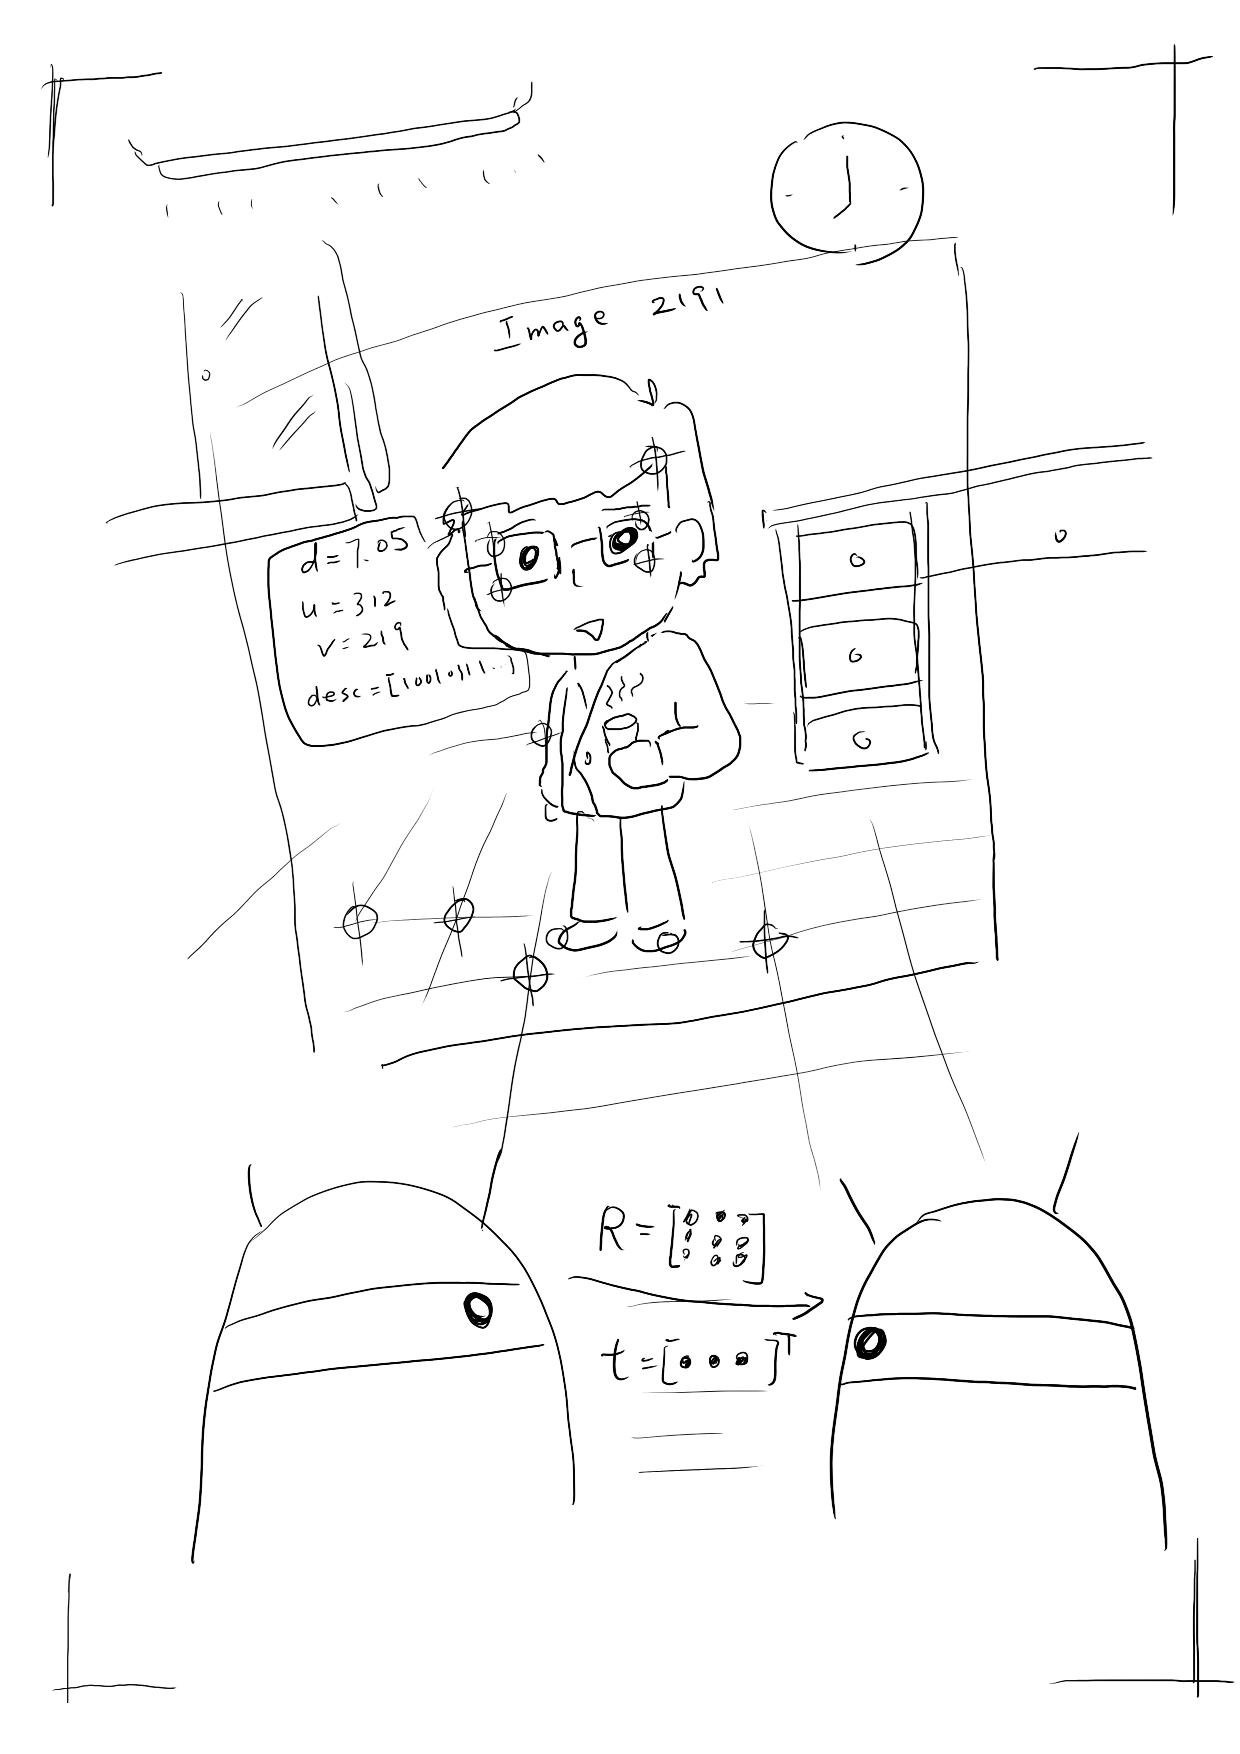
\includepdf{resources/other/ch7.pdf}

\newpage

\section{Feature Method}
In chapter~\ref{cpt:2}, we said that a SLAM system can be divided into frontend and backend, where the frontend is also called visual odometry (VO). VO estimates the rough camera movement based on the consecutive images' information and provides a good initial value for the backend. VO algorithms are mainly divided into two categories: feature method and direct method. The frontend based on the features has been considered the mainstream of VO for a long time (even until now). It performs well thanks to its stability and insensitivity to lighting and dynamic objects. The feature method is relatively mature at present. This chapter will start with the feature method, learn how to extract and match image feature points, and then estimate the camera motion and scene structure between two frames to realize visual odometry between two frames. This type of algorithm is sometimes called two-view geometry.

The core problem of VO is how to estimate camera motion based on adjacent images. However, the image itself is a numerical matrix encoding brightness and color. The numbers in the matrix are abstract, and it is very difficult to compute the motion directly from the pixel level. Therefore, it is more convenient to do this: First, select some representative features from the image. These points will remain the same after a small change in the camera's angle of view. So we are able to find the same points in each image. Then, based on these points, we can investigate the problem of camera pose estimation and the 3D positions of these points. In the classic SLAM model, we call these points the landmarks. In visual SLAM, they are referred to as image features.

On Wikipedia, image features are defined as a set of information related to computing tasks. The computing tasks depend on the specific application~\cite{wiki:featurecv}. Briefly speaking, the feature is another digital expression of image information. A good set of features is crucial to the final performance on the specified task, so researchers have comprehensive work on the features for many years. Digital images are stored in a computer as a gray value matrix, so at the simplest, a single image pixel can also be considered a feature. However, in visual odometry, we hope that feature points remain stable after the camera moves, and the gray value is severely affected by illumination, deformation, and object material. It varies significantly between different images and is not stable enough. Ideally, when the scene and camera angle of view changes slightly, the algorithm can also determine from the images which places refer to the same point. Therefore, the gray value alone is not feasible. We need to extract better features from the image.

We can say that the feature points are some special places in the image. Taking \autoref{fig:corner-feature}~ as an example, we can see the corners, edges, and blocks as representative places in the image. It is easy for us to correctly point out that the same corner point appears in two images, whereas pointing out the same edge is slightly more difficult because the image patches are similar when moving along the edges. It is even harder for the blocks. We found that the corners and edges in the image are more \textit{special} than pixels, and they are more distinguished between different images. Therefore, an intuitive way to extract features is to identify corners between different images and determine their correspondence. In this approach, the corners are the so-called features. There are many corner extraction algorithms, such as Harris corner~\cite{Harris1988}, FAST corner {\cite{Rosten2006}}, GFTT corner  {\cite{Shi1994}}, etc. Most of them were proposed before 2000.

However, in the majority of applications, a single corner still cannot meet our needs. For example, a place that appears to be a corner from a long distance may not be viewed as a corner when the camera steps in. When the camera rotates, the appearance of the corner points will change, and it is not easy for us to recognize that they are the same corner point. For this reason, researchers in the field of computer vision have designed many more stable local image features during years of research, such as the SIFT~\cite{Lowe2004}, SURF {\cite{Bay2006}} , ORB {\cite{Rublee2011}}, etc. Compared with simple corner points, these handcrafted features should have the following properties:

\begin{enumerate}
\item \textbf{Repeatability}: The same feature can be found in different images.
\item \textbf{Distinctiveness}: Different features have different expressions.
\item \textbf{Efficiency}: In the same image, the number of feature points should be far smaller than the number of pixels.
\item \textbf{Locality}: The feature is only related to a small image area.
\end{enumerate}

\begin{figure}[!ht]
    \centering
    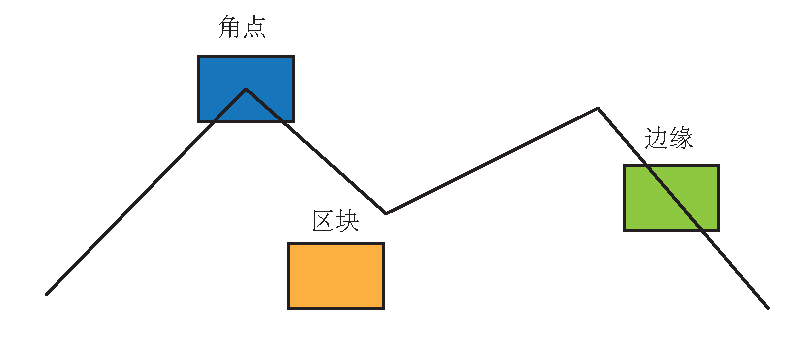
\includegraphics[width=0.8\linewidth]{vo1/corner-flat-line}
    \caption{Corners, edges and blocks can be used as image features.}
    \label{fig:corner-feature}
\end{figure}

A feature point is composed of two parts: \textit{key point} and \textit{descriptor}. For example, when we say ``calculate SIFT feature points in an image'', we mean ``extract SIFT key points and calculate the SIFT descriptors``. The key point refers to the 2D position of the feature point. Some types of key points also hold other information, such as the orientation and size. According to some handcrafted rules, the descriptor is usually a vector, describing the information of the pixels around the key point. The descriptor should be designed according to the principle that features with similar appearance should have similar descriptors. Therefore, as long as the two features' descriptors are close in vector space, they can be considered the same feature. 

Historically, researchers put forward many image features. Some of them are very accurate and robust. They still have similar expressions under camera movement and lighting changes, and consequentially they might require a large amount of calculation. Among them, SIFT (Scale-Invariant Feature Transform) is one of the most classic. To fully consider the changes in illumination, scale, and rotation during the image transformation, the SIFT comes with a considerable amount of calculation. The extraction and matching of image features is only a part compared to the entire SLAM process. Until now (2016), CPUs equipped on PCs cannot achieve real-time to calculate the SIFT features for localization and mapping \footnote{Real-time means the speed of 30Hz. }. So, we rarely use this luxury image feature in SLAM.

Some other features exchange accuracy and robustness for the calculation speed increase. For example, the FAST keypoint is a key point that is extremely fast to calculate (note the expression of keypoint here, which means that it has no descriptor), while the ORB (Oriented FAST and Rotated BRIEF) feature is currently widely used for real-time image feature extraction. It solves the problem that the FAST detector  {\cite{Rosten2006}} does not have descriptors and uses the extremely fast binary descriptor BRIEF {\cite{calonder2010brief}} to make the whole image feature extraction process accelerate greatly. According to the author's experiment in the paper, extracting about 1000 feature points in the same image takes about 15.3ms for ORB, 217.3ms for SURF, and 5228.7ms for SIFT. It can be seen that ORB made a significant boost in speed while maintaining the features of rotation and scale invariance. It is a good choice for SLAM with high real-time requirements.

Most feature extractions have good parallelism and can be accelerated by GPU and other devices. SIFT accelerated by GPU can meet real-time requirements. However, the inclusion of a GPU will increase the cost of the entire SLAM system \footnote{But now we have many cheap embedded GPU chips, so it may not be an issue anymore.}. Whether the resulting performance improvement is sufficient to offset the computational cost requires careful consideration by the system designer.

Obviously, there are a large number of feature points in the field of computer vision, and we cannot introduce them one by one in the book. In the current SLAM scheme, ORB is a fair trade-off between quality and performance. Therefore, we take ORB as an example to introduce the entire process of extracting features. If readers are interested in feature extraction and matching algorithms, we recommend reading related books in this area~\cite{Nixon2012}.

\subsection{ORB Feature}

ORB features are also composed of two parts: \textit{ORB key points} and \textit{ORB descriptor}. Its key point is called ``oriented FAST'', which is an improved version of the FAST. We will introduce what the FAST corner below is. Its descriptor is called BRIEF (Binary Robust Independent Elementary Feature). Therefore, the extraction of ORB features is divided into the following two steps:
\begin{enumerate}
\item FAST corner point extraction: find the corner point in the image. Compared with the original FAST, the main direction of the feature points is calculated in ORB, making the subsequent BRIEF descriptor rotation-invariant.
\item BRIEF descriptor: describe the surrounding image area where the feature points were extracted in the previous step. ORB has made some improvements to BRIEF, mainly referring to utilizing the previously calculated direction.
\end{enumerate}

Next, we will introduce FAST and BRIEF, respectively.

\subsubsection{The FAST Key Point}
FAST is a kind of corner point, which mainly detects the local grayscale changes and is known for its fast speed. Its main idea is: if a pixel is very different from the neighboring pixels (too bright or too dark), it is more likely to be a corner point. Compared with other corner detection algorithms, FAST only needs to compare the pixels' brightness. Its entire procedure is as follows (see \autoref{fig:fastcorner}~):

\begin{enumerate}
\item Select pixel $p$ in the image, assuming its brightness as $I_{p}$
\item Set a threshold $T$ (for example, 20\% of $I_{p}$).
\item Take the pixel $p$ as the center, and select the 16 pixels on a circle with a radius of 3.
\item If there are consecutive $N$ points on the selected circle whose brightness is greater than $I_{p}+T$ or less than $I_{p}-T$, then the central pixel $p$ can be considered a feature point. $N$ usually takes 12, which is FAST-12. Other commonly used $N$ values are 9 and 11, called FAST-9 and FAST-11, respectively).
\item Iterate through the above four steps on each pixel.
\end{enumerate}

In the FAST-12 algorithm, to speed up, we can check the brightness of the 1, 5, 9, and 13 pixels on the circle to quickly exclude many pixels that are not corner points. Only when three of these four pixels are all greater than $I_{p}+T$ or less than $I_{p}-T$, the current pixel may potentially be a corner point. Otherwise, it should be directly excluded. Such a pre-processing operation greatly accelerates FAST corner detection. Also, the original FAST corners are often clustered, meaning a lot of FAST corners may present in the same area. Therefore, after the initial detection, non-maximal suppression is required. Only corner points with the maximum response in a specific location will be retained to avoid the corners concentrating.

\begin{figure}[!ht]
	\centering
	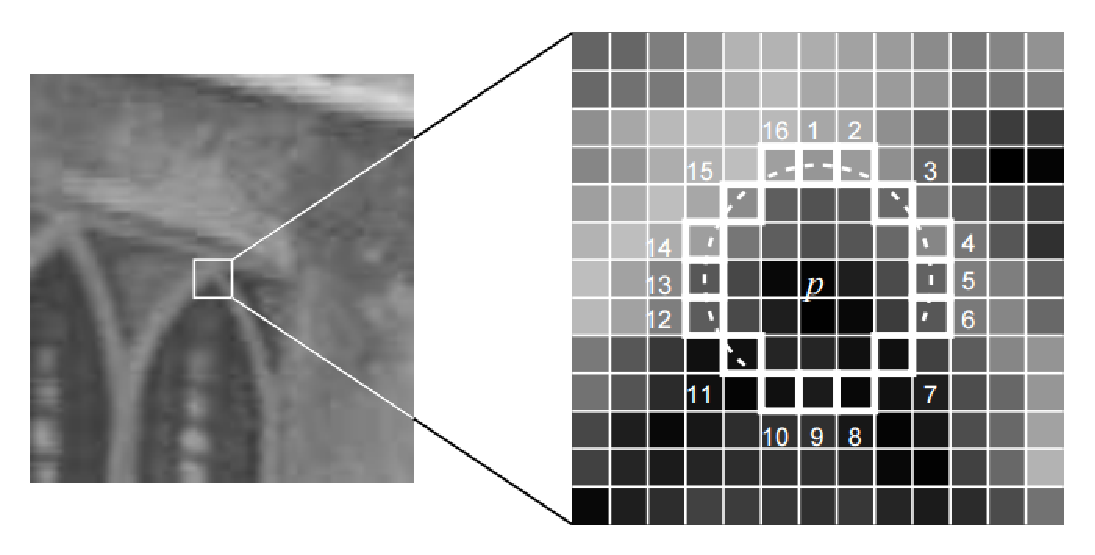
\includegraphics[width=0.9\linewidth]{vo1/fast-corner}
	\caption{FAST key points {\cite{Rosten2006}}. This figure is from OpenCV's document.}
	\label{fig:fastcorner}
\end{figure}

The calculation of FAST feature points only compares the brightness difference between pixels, thus the speed is very fast, but it suffers from lousy repeatability and uneven distribution. Moreover, FAST corner points do not include direction information. Because it fixed the radius of the circle as 3, there is also a scaling problem: a place that looks like a corner from a distance may not be a corner when it comes close. To solve those, ORB adds the description of scale and rotation. The scale invariance is achieved by the image pyramid \footnote{Pyramid refers to the downsampling of images at different levels to obtain images with different resolutions. } and detect corner points on each layer. The rotation of features is realized by the intensity centroid method.

An image pyramid is a common approach in computer vision. For a schema, see \autoref{fig:pyramid}. The bottom of the pyramid is the original image. For each layer up, the image is scaled with a fixed ratio so that we have images of different resolutions. The smaller image can be seen as a scene viewed from a distance. In the feature matching algorithm, we can match images on different layers to achieve scale invariance. For example, if the camera moves backward, we should find a match in the upper layer of the previous image pyramid and the lower layer of the next image.

\begin{figure}[!t]
    \centering
    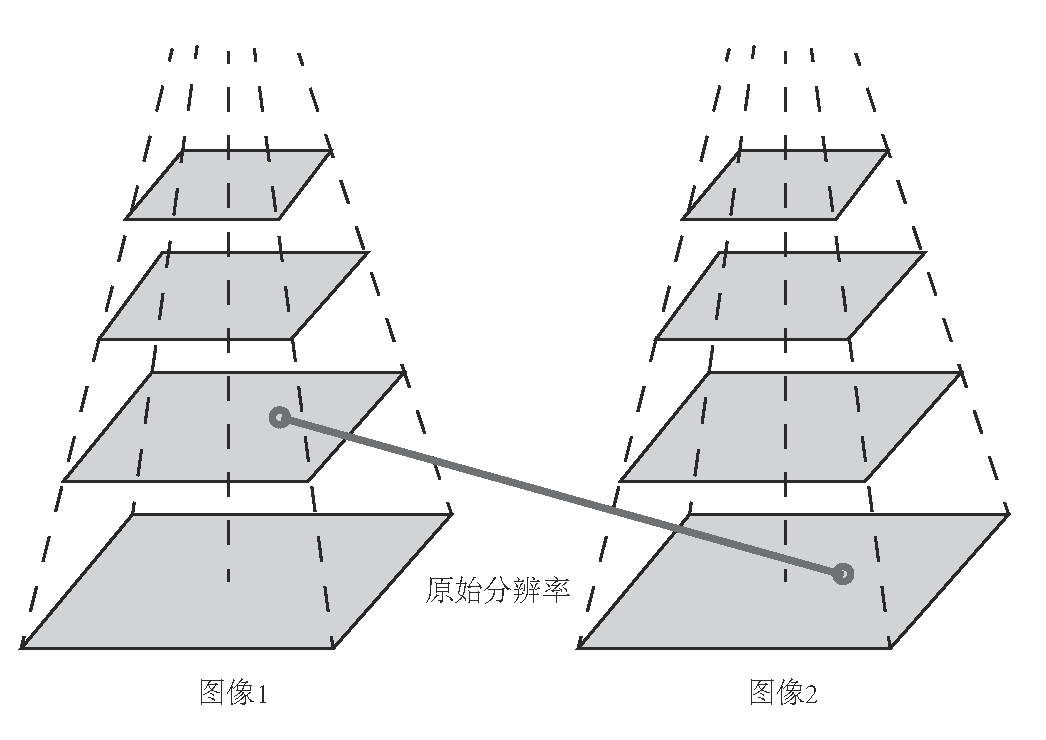
\includegraphics[width=0.9\linewidth]{vo1/pyramid}\\
    \caption{Use pyramids to match images at different resolutions.}
    \label{fig:pyramid}
\end{figure}

In terms of rotation, we calculate the gray centroid of the image near the feature point. The so-called centroid refers to the gray value of the image block as the center of weight. The specific steps are as follows {\cite{Rosin1999}}:

\begin{enumerate}
\item In a small image block $B$, define the moment of the image block as:
\[
m_{pq}=\sum_{x,y \in B}x^{p}y^{q}I(x,y), \quad p, q = \{0,1\}.
\]
\item Calculate the centroid of the image block by the moment:
\[
C=\left(\frac{m_{10}}{m_{00}},\frac{m_{01}}{m_{00}}\right).
\]
\item Connect the geometric center $O$ and the centroid $C$ of the image block to get a direction vector $\overrightarrow{OC}$, so the direction of the feature point can be defined as:
\[
\theta = \arctan(m_{01}/m_{10}).
\]
\end{enumerate}
FAST corner points have a description of scale and rotation, which significantly improves the robustness of their representation between different images. This improved FAST is called oriented FAST in ORB.

\subsubsection{BRIEF Descriptor}
After extracting the Oriented FAST key points, we calculate the descriptor for each point. ORB uses an improved BRIEF feature description. Let's first introduce what BRIEF is.

BRIEF is a binary descriptor. Its description vector consists of many zeros and ones, which encode the size relationship between two random pixels near the key point (such as $p$ and $q$): If $p$ is greater than $q$, then take 1, otherwise take 0. If we take 128 such $p,q$ pairs, we will finally get a 128-dimensional vector  {\cite{calonder2010brief}} consisting of 0s and 1s. The BRIEF implements the comparison of randomly selected points, which is very fast. Since it expresses in binary, it is also very convenient to store and suitable for real-time image matching. The original BRIEF descriptor does not have rotation invariance, so it is easy to get lost when the image is rotated. The ORB calculates the direction of the key points in the FAST feature point extraction stage. The direction information can be used to calculate the Steer BRIEF feature after the rotation so that the ORB descriptor has better rotation invariance.

Due to the consideration of rotation and scaling, the ORB performs well under translation, rotation, and scaling. Meanwhile, the combination of FAST and BRIEF is very efficient, which makes ORB features very popular in real-time SLAM. In \autoref{fig:ORB}~, we show the result of extracting ORB from an image. In the following, we will move on to feature matching between different images.

\begin{figure}[!htp]
    \centering
    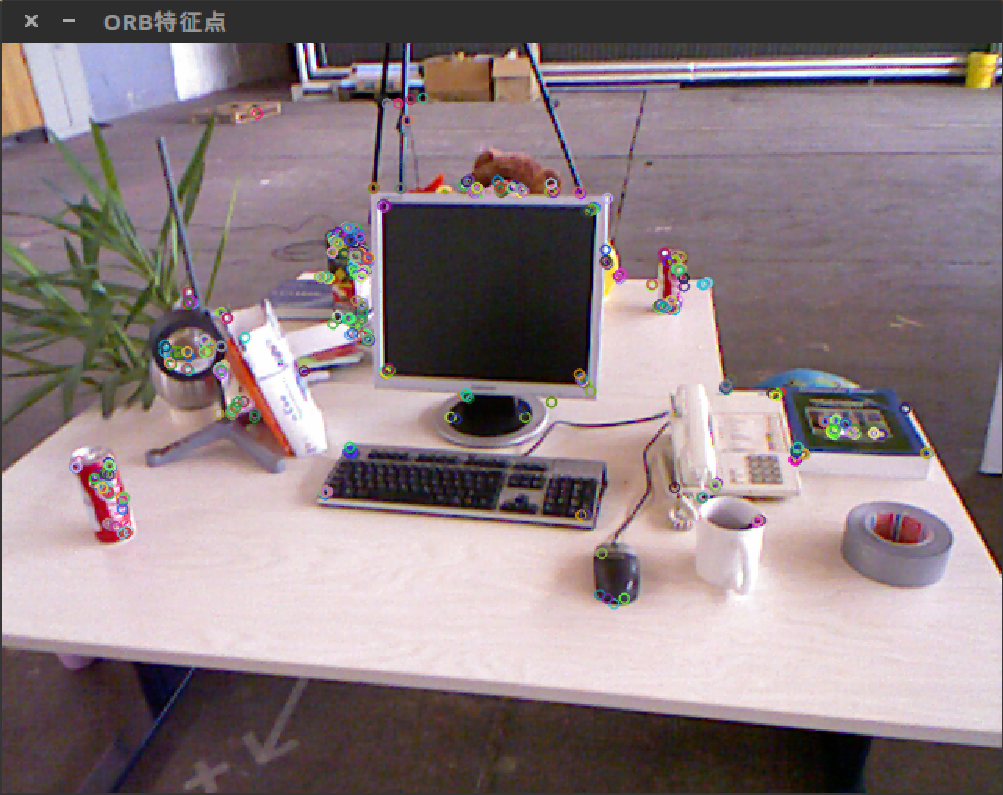
\includegraphics[width=0.9\linewidth]{vo1/feature}\\
    \caption{ORB feature points detected by OpenCV.}
    \label{fig:ORB}
\end{figure}

\subsection{Feature Matching}

Feature matching is a critical step in visual SLAM (\ref{fig:feature-matching}). Broadly speaking, feature matching solves the data association problem in SLAM, that is, to determine the view correspondence between the landmarks (feature points) and the landmarks (feature points) seen before. By accurately matching the descriptors between images or between images and maps, we can reduce a lot of work for subsequent pose estimation and optimization operations. However, due to the locality of image features, mismatches are common and have not been effectively resolved for a long time. It has become a significant bottleneck to improve the performance of visual SLAM. It is somehow due to repeated textures in the scene, making the feature descriptions very similar. Under this circumstance, it is hard to resolve the mismatch by using local features only.

\begin{figure}[!htp]
    \centering
    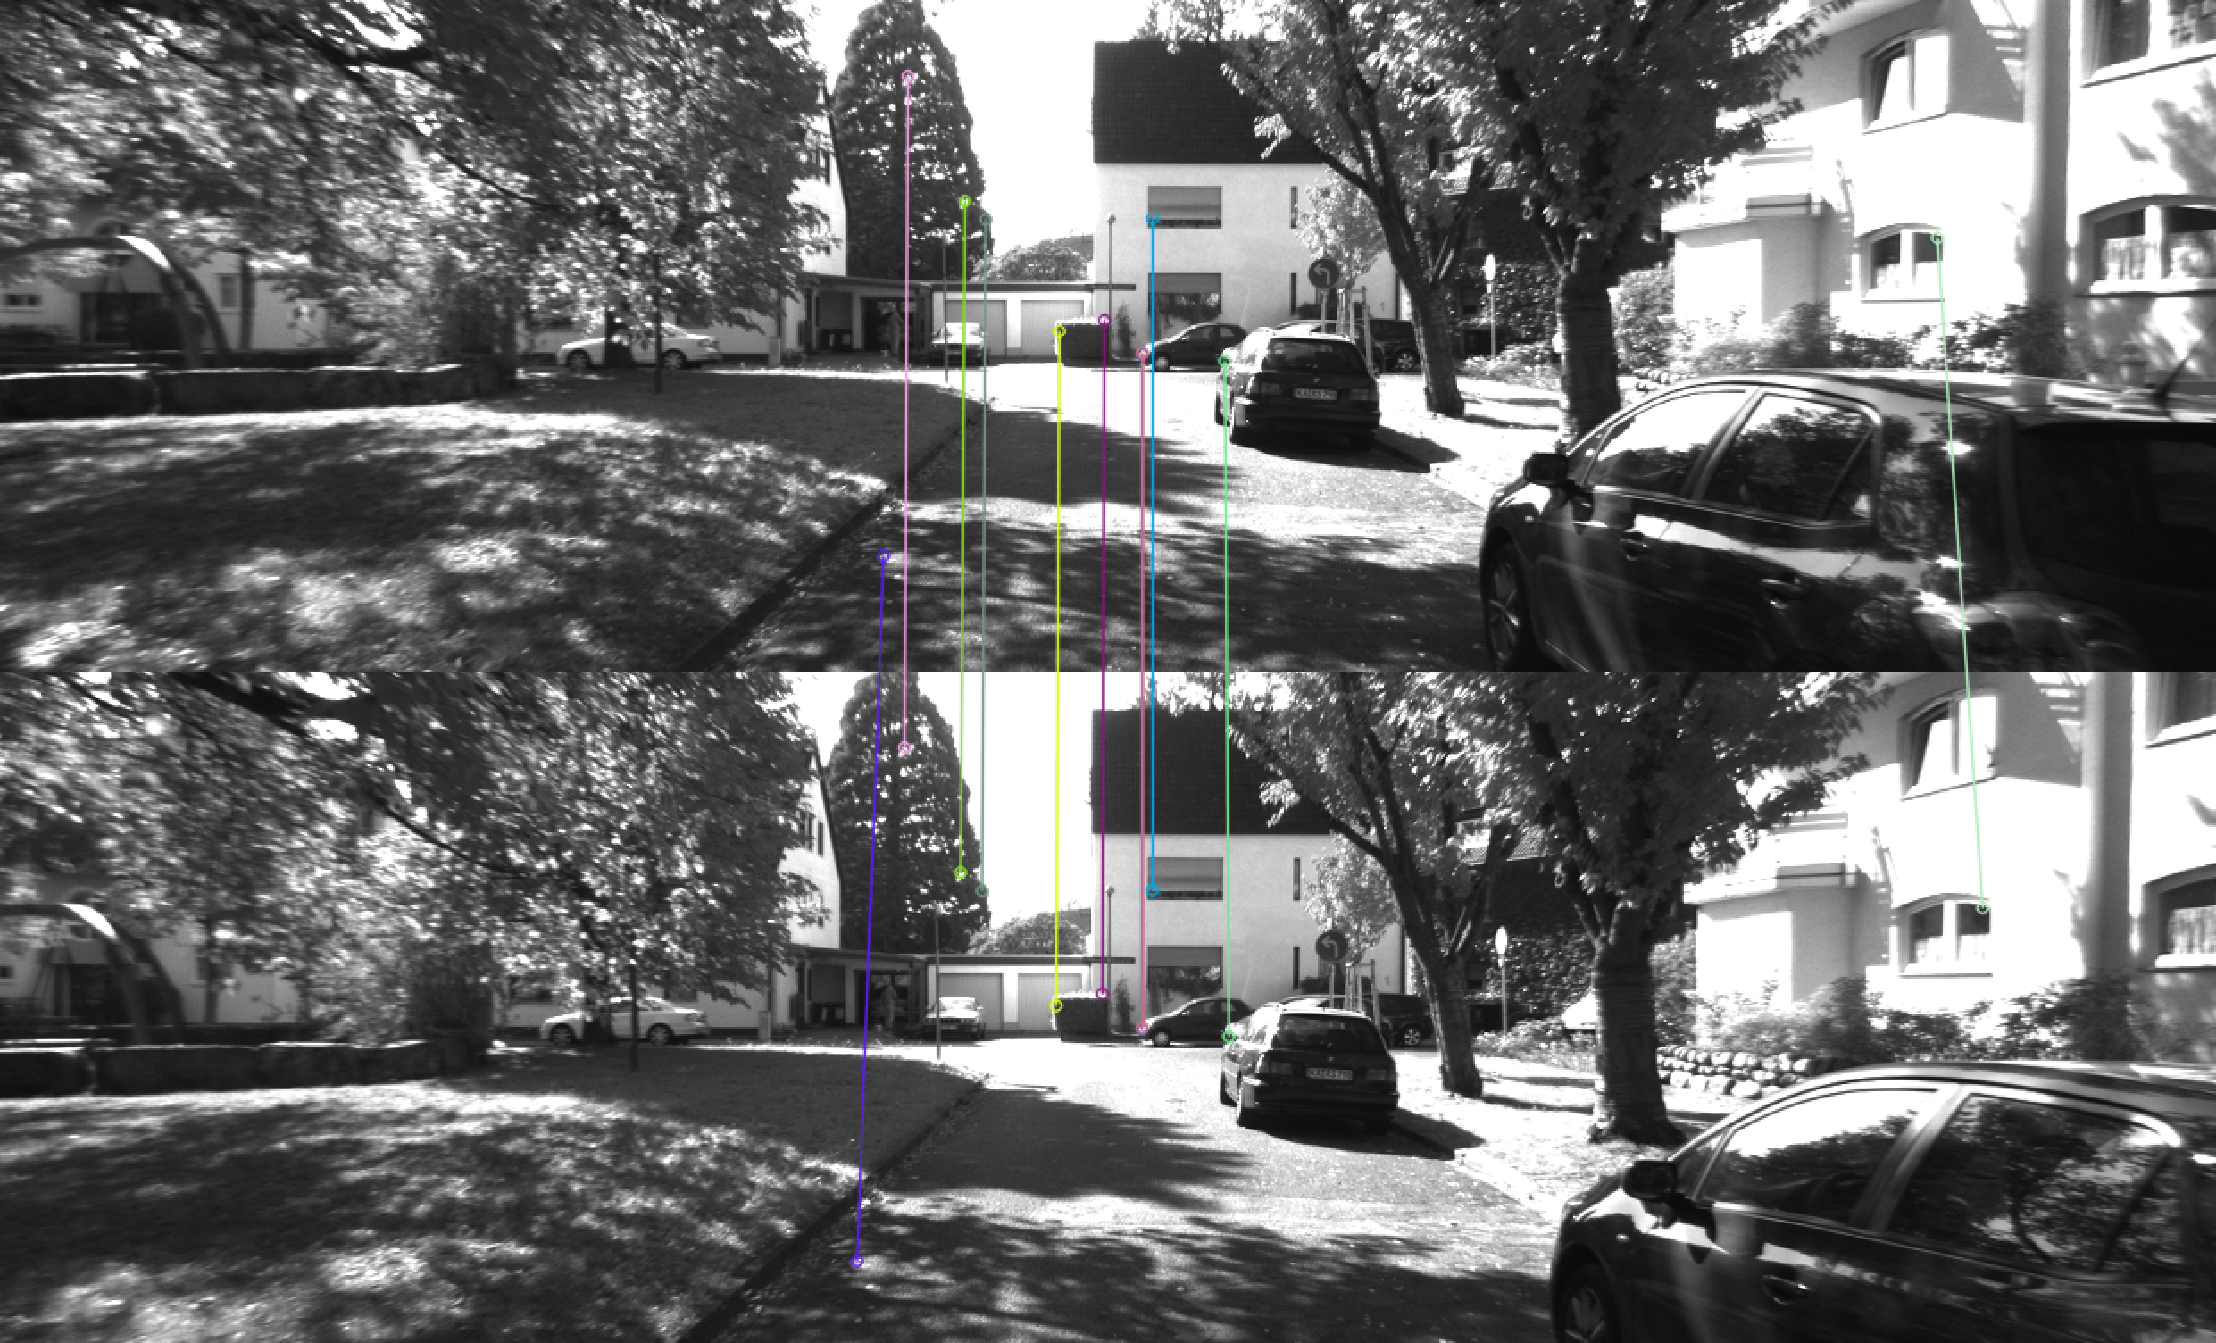
\includegraphics[width=0.9\linewidth]{vo1/feature-matching}
    \caption{Feature matching between two images.}
    \label{fig:feature-matching}
\end{figure}

However, let's first assume the matching is correct and then go back to discuss the mismatch problem. Consider images at two moments. Assume features $x_{t}^{m}, m=1,2,...,M$ are extracted in the image $I_{t}$, and $x_{t+1}^{n}, n=1,2,...,N$ in $I_{t+1}$ . How do we find the correspondence between these two sets? The simplest feature matching method is the brute-force matcher, which measures the distance between each pair of the features $x_{t}^{m}$ and all $x_{t+1}^{n}$ descriptors. Then sort the matching distance, and take the closest one as the matching point. The descriptor distance indicates the degree of similarity of two features. In practice, different distance metric norms can be used. For descriptors of floating-point type, using Euclidean distance to measure is a good choice. For binary descriptors (such as BRIEF), we often use Hamming distance as a metric. The Hamming distance between two binary vectors refers to the number of different digits.

When the number of feature points is large, the brute force matching's computational complexity will become too expensive, especially when you want to match a frame to a map. This does not meet our real-time requirements in SLAM. The Fast Approximate Nearest Neighbor (FLANN) algorithm is more suitable in this case. Since these matching algorithms' theory is mature and the implementation has already been integrated into OpenCV, the technical details will not be described here. Interested readers can refer to the literature~\cite{Muja2009}.In engineering, we can also limit the search range of the brute-force method to achieve real-time performance.

\section{Practice: Feature Extraction and Matching}
\begin{figure}[!htp]
	\centering
	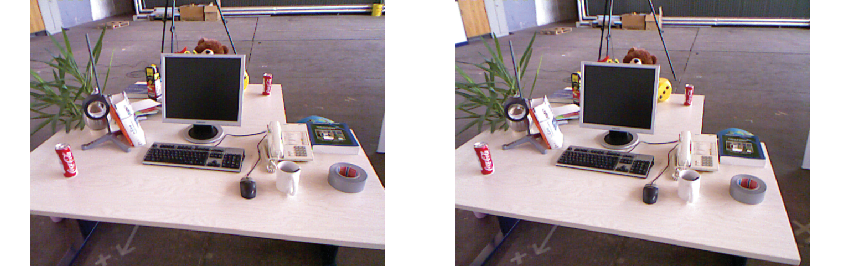
\includegraphics[width=0.9\linewidth]{vo1/exp1-images.pdf}
	\caption{Two images used in the practice.}
	\label{fig:exp1-images}
\end{figure}

OpenCV has integrated most of the image features, and we can easily use them by function calls. Let's demonstrate two examples here. In the first one, we show the use of OpenCV for feature matching of ORB; in the second, we explain how to write an ORB feature from scratch based on the principles. Through the practice, readers will have a deeper understanding of the ORB calculation process. Then other features can be done analogously.

\subsection{ORB Features in OpenCV}
First, we call OpenCV to extract and match ORB. We prepared two images for this practice, 1.png and 2.png under ``slambook2/ch7/'', as shown in \autoref{fig:exp1-images}~. They are two images from the public dataset~\cite{Sturm2012}. We can see a slight movement of the camera. The procedure in this section demonstrates how to extract ORB features and perform matching. In the next section, we will show how to use matching results to estimate camera motion.

The following program demonstrates how to use ORB:
\begin{lstlisting}[language=c++,caption=slambook2/ch7/orb_cv.cpp]
#include <iostream>
#include <opencv2/core/core.hpp>
#include <opencv2/features2d/features2d.hpp>
#include <opencv2/highgui/highgui.hpp>
#include <chrono>

using namespace std;
using namespace cv;

int main(int argc, char **argv) {
	if (argc != 3) {
		cout << "usage: feature_extraction img1 img2" << endl;
		return 1;
	}
	//-- read images
	Mat img_1 = imread(argv[1], CV_LOAD_IMAGE_COLOR);
	Mat img_2 = imread(argv[2], CV_LOAD_IMAGE_COLOR);
	assert(img_1.data != nullptr && img_2.data != nullptr);
	
	//-- initialization
	std::vector<KeyPoint> keypoints_1, keypoints_2;
	Mat descriptors_1, descriptors_2;
	Ptr<FeatureDetector> detector = ORB::create();
	Ptr<DescriptorExtractor> descriptor = ORB::create();
	Ptr<DescriptorMatcher> matcher = DescriptorMatcher::create("BruteForce-Hamming");
	
	//-- detect  Oriented FAST
	chrono::steady_clock::time_point t1 = chrono::steady_clock::now();
	detector->detect(img_1, keypoints_1);
	detector->detect(img_2, keypoints_2);
	
	//-- compute BRIEF descriptor
	descriptor->compute(img_1, keypoints_1, descriptors_1);
	descriptor->compute(img_2, keypoints_2, descriptors_2);
	chrono::steady_clock::time_point t2 = chrono::steady_clock::now();
	chrono::duration<double> time_used = chrono::duration_cast<chrono::duration<double>>(t2 - t1);
	cout << "extract ORB cost = " << time_used.count() << " seconds. " << endl;
	
	Mat outimg1;
	drawKeypoints(img_1, keypoints_1, outimg1, Scalar::all(-1), DrawMatchesFlags::DEFAULT);
	imshow("ORB features", outimg1);
	
	//-- use Hamming distance to match the features
	vector<DMatch> matches;
	t1 = chrono::steady_clock::now();
	matcher->match(descriptors_1, descriptors_2, matches);
	t2 = chrono::steady_clock::now();
	time_used = chrono::duration_cast<chrono::duration<double>>(t2 - t1);
	cout << "match ORB cost = " << time_used.count() << " seconds. " << endl;
	
	//-- sort and remove the outliers
	// min and max distance
	auto min_max = minmax_element(matches.begin(), matches.end(),
		[](const DMatch &m1, const DMatch &m2) { return m1.distance < m2.distance; });
	double min_dist = min_max.first->distance;
	double max_dist = min_max.second->distance;
	
	printf("-- Max dist : %f \n", max_dist);
	printf("-- Min dist : %f \n", min_dist);
	
	// remove the bad matching
	std::vector<DMatch> good_matches;
	for (int i = 0; i < descriptors_1.rows; i++) {
		if (matches[i].distance <= max(2 * min_dist, 30.0)) {
			good_matches.push_back(matches[i]);
		}
	}
	
	//-- draw the results
	Mat img_match;
	Mat img_goodmatch;
	drawMatches(img_1, keypoints_1, img_2, keypoints_2, matches, img_match);
	drawMatches(img_1, keypoints_1, img_2, keypoints_2, good_matches, img_goodmatch);
	imshow("all matches", img_match);
	imshow("good matches", img_goodmatch);
	waitKey(0);
	
	return 0;
}
\end{lstlisting}

Run this program (you need to enter the paths of two images manually). The screen output should be like this:
\begin{lstlisting}[language=sh,caption=Terminal input:]
% build/orb_cv 1.png 2.png
extract ORB cost = 0.0229183 seconds. 
match ORB cost = 0.000751868 seconds.
-- Max dist : 95.000000 
-- Min dist : 4.000000 
\end{lstlisting}

\autoref{fig:exp1-results}~shows the results of the example. We see a large number of false matches before the filtering. After removing the bad matches, most of the remaining matches are correct. Here, we followed an empirical rule in engineering that good matches are selected from where the Hamming distance is less than twice the minimum distance. It may not have a theoretical explanation but just an engineering trick. However, although we can select out the correct matches in the example image, we still cannot guarantee that the remaining matches are correct. Therefore, during the motion estimation step, it is necessary to consider those mismatches. ORB extraction took 22.9 milliseconds (two images) on my machine, and matching took 0.75 milliseconds. It can be seen that most of the calculation is spent on feature extraction.

\begin{figure}[!htp]
	\centering
	\includegraphics[width=1.0\linewidth]{vo1/exp1-result}
	\caption{Feature extraction and matching results.}
	\label{fig:exp1-results} 
\end{figure}

\subsection{ORB Features from Scratch}
Below we show the method of coding ORB features from scratch. Since the code is a bit long, only a snippet is shown here. Readers are recommended to obtain the rest from the GitHub codebase.
\begin{lstlisting}[language=c++,caption=slambook2/ch7/orb_self.cpp (part)]
typedef vector<uint32_t> DescType;
// ... omit some image loading and testing code
// compute the descriptor
void ComputeORB(const cv::Mat &img, vector<cv::key point> &key points, vector<DescType> &descriptors) {
    const int half_patch_size = 8;
    const int half_boundary = 16;
    int bad_points = 0;
    for (auto &kp: key points) {
        if (kp.pt.x < half_boundary || kp.pt.y < half_boundary ||
        kp.pt.x >= img.cols - half_boundary || kp.pt.y >= img.rows - half_boundary) {
            // outside
            bad_points++;
            descriptors.push_back({});
            continue;
        }
    
        float m01 = 0, m10 = 0;
        for (int dx = -half_patch_size; dx < half_patch_size; ++dx) {
            for (int dy = -half_patch_size; dy < half_patch_size; ++dy) {
                uchar pixel = img.at<uchar>(kp.pt.y + dy, kp.pt.x + dx);
                m01 += dx * pixel;
                m10 += dy * pixel;
            }
        }
    
        // angle should be arc tan(m01/m10);
        float m_sqrt = sqrt(m01 * m01 + m10 * m10);
        float sin_theta = m01 / m_sqrt;
        float cos_theta = m10 / m_sqrt;
        
        // compute the angle of this point
        DescType desc(8, 0);
        for (int i = 0; i < 8; i++) {
            uint32_t d = 0;
            for (int k = 0; k < 32; k++) {
                int idx_pq = i * 8 + k;
                cv::Point2f p(ORB_pattern[idx_pq * 4], ORB_pattern[idx_pq * 4 + 1]);
                cv::Point2f q(ORB_pattern[idx_pq * 4 + 2], ORB_pattern[idx_pq * 4 + 3]);
        
                // rotate with theta
                cv::Point2f pp = cv::Point2f(cos_theta * p.x - sin_theta * p.y, sin_theta * p.x + cos_theta * p.y) + kp.pt;
                cv::Point2f qq = cv::Point2f(cos_theta * q.x - sin_theta * q.y, sin_theta * q.x + cos_theta * q.y) + kp.pt;	
                
                // compare pp and qq
                if (img.at<uchar>(pp.y, pp.x) < img.at<uchar>(qq.y, qq.x)) {
                    d |= 1 << k;
                }
            }
            desc[i] = d;
        }
        descriptors.push_back(desc);
    }
    
    cout << "bad/total: " << bad_points << "/" << key points.size() << endl;
}

// brute-force matching
void BfMatch(
    const vector<DescType> &desc1, const vector<DescType> &desc2, vector<cv::DMatch> &matches) {
    const int d_max = 40;
    
    for (size_t i1 = 0; i1 < desc1.size(); ++i1) {
        if (desc1[i1].empty()) continue;
        cv::DMatch m{i1, 0, 256};
        for (size_t i2 = 0; i2 < desc2.size(); ++i2) {
            if (desc2[i2].empty()) continue;
            int distance = 0;
            for (int k = 0; k < 8; k++) {
                distance += _mm_popcnt_u32(desc1[i1][k] ^desc2[i2][k]);
            }
            if (distance < d_max && distance < m.distance) {
                m.distance = distance;
                m.trainIdx = i2;
            }
        }
        if (m.distance < d_max) {
            matches.push_back(m);
        }
    }
}
\end{lstlisting}
We only show the ORB calculation and matching code. In the calculation, we use 256-bit binary description, which corresponds to 8 32-bit unsigned int data expressed as DescType with typedef. Then, we calculate the FAST feature point's angle according to the principle introduced above and then use the angle to calculate the descriptor. To accelerate, some complicated calculations, such as $\arctan$, $\sin$, and $\cos$, are worked around by the principle of trigonometric functions. In the BfMatch function, we also use the \_mm\_popcnt\_u32 function in the SSE instruction set to calculate the number of 1s in an unsigned int, which is used to achieve the effect of calculating the Hamming distance. The result of this program is as follows, and the matching result is shown in \autoref{fig:matches}:

\begin{lstlisting}[language=sh,caption=Terminal output:]
bad/total: 43/638
bad/total: 8/595
extract ORB cost = 0.00390721 seconds.
match ORB cost = 0.000862984 seconds.
matches: 51
\end{lstlisting}

\begin{figure}[!htp]
    \centering
    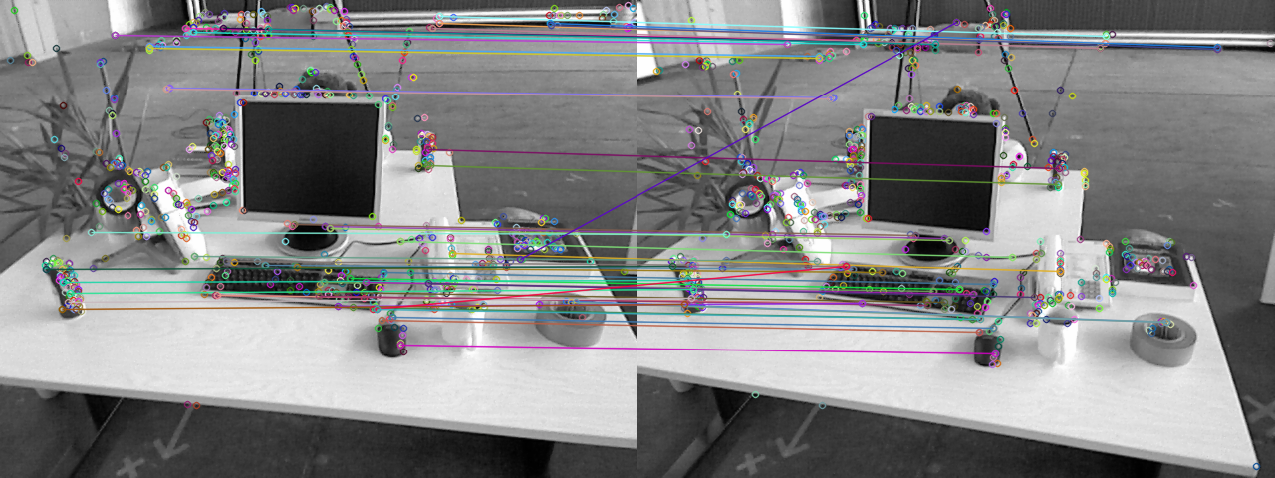
\includegraphics[width=0.8\linewidth]{vo1/matches}
    \caption{Matching Result}
    \label{fig:matches}
\end{figure}

In this program, ORB extraction takes 3.9 milliseconds, and the matching takes only 0.86 milliseconds. Through some simple modifications in implementation, we accelerated the extraction of ORB by 5.8 times. Note that compiling this program requires your CPU to support the SSE instruction set, which should be already supported on most modern PC CPUs. If we can further parallelize the feature extraction, the algorithm can be further accelerated.

\subsection{Calculate the Camera Motion}
Now, we have key points matching. In the next step, we need to estimate the camera's motion based on the matching. It is totally different for different camera settings (or the information available for the calculation):

\begin{enumerate}
	\item When the camera is monocular, we only know the 2D pixel coordinates, so the problem is to estimate the motion according to two sets of 2D points. This problem is solved by \textit{epipolar geometry}.
	\item When the camera is binocular, RGB-D, or the distance is obtained by some method, then the problem is to estimate the motion according to two sets of 3D points. This problem is usually solved by ICP.
	\item If one set is 3D and one set is 2D, we get some 3D points and their projection positions on the camera, and we can also estimate the camera's pose. This problem is solved by \textit{PnP}.
\end{enumerate}

The following sections will introduce camera motion estimation in these three situations. We will start from the 2D-2D case with the least information and see how it is dealt with and troublesome problems.

\section{2D−2D: Epipolar Geometry}
\label{sec:epipolar-geometry}

\subsection{Epipolar Constraints}

Suppose we have a pair of matched feature points from two images, as shown in \autoref{fig:doubleview}~. If there are several pairs of such matching points, the camera motion between the two frames can be recovered through the correspondence between these two-dimensional image points. How many pairs do we need? We will see later. Let's first take a look at the geometric relationship between the matching points in the two images.

\begin{figure}[!htp]
	\centering
	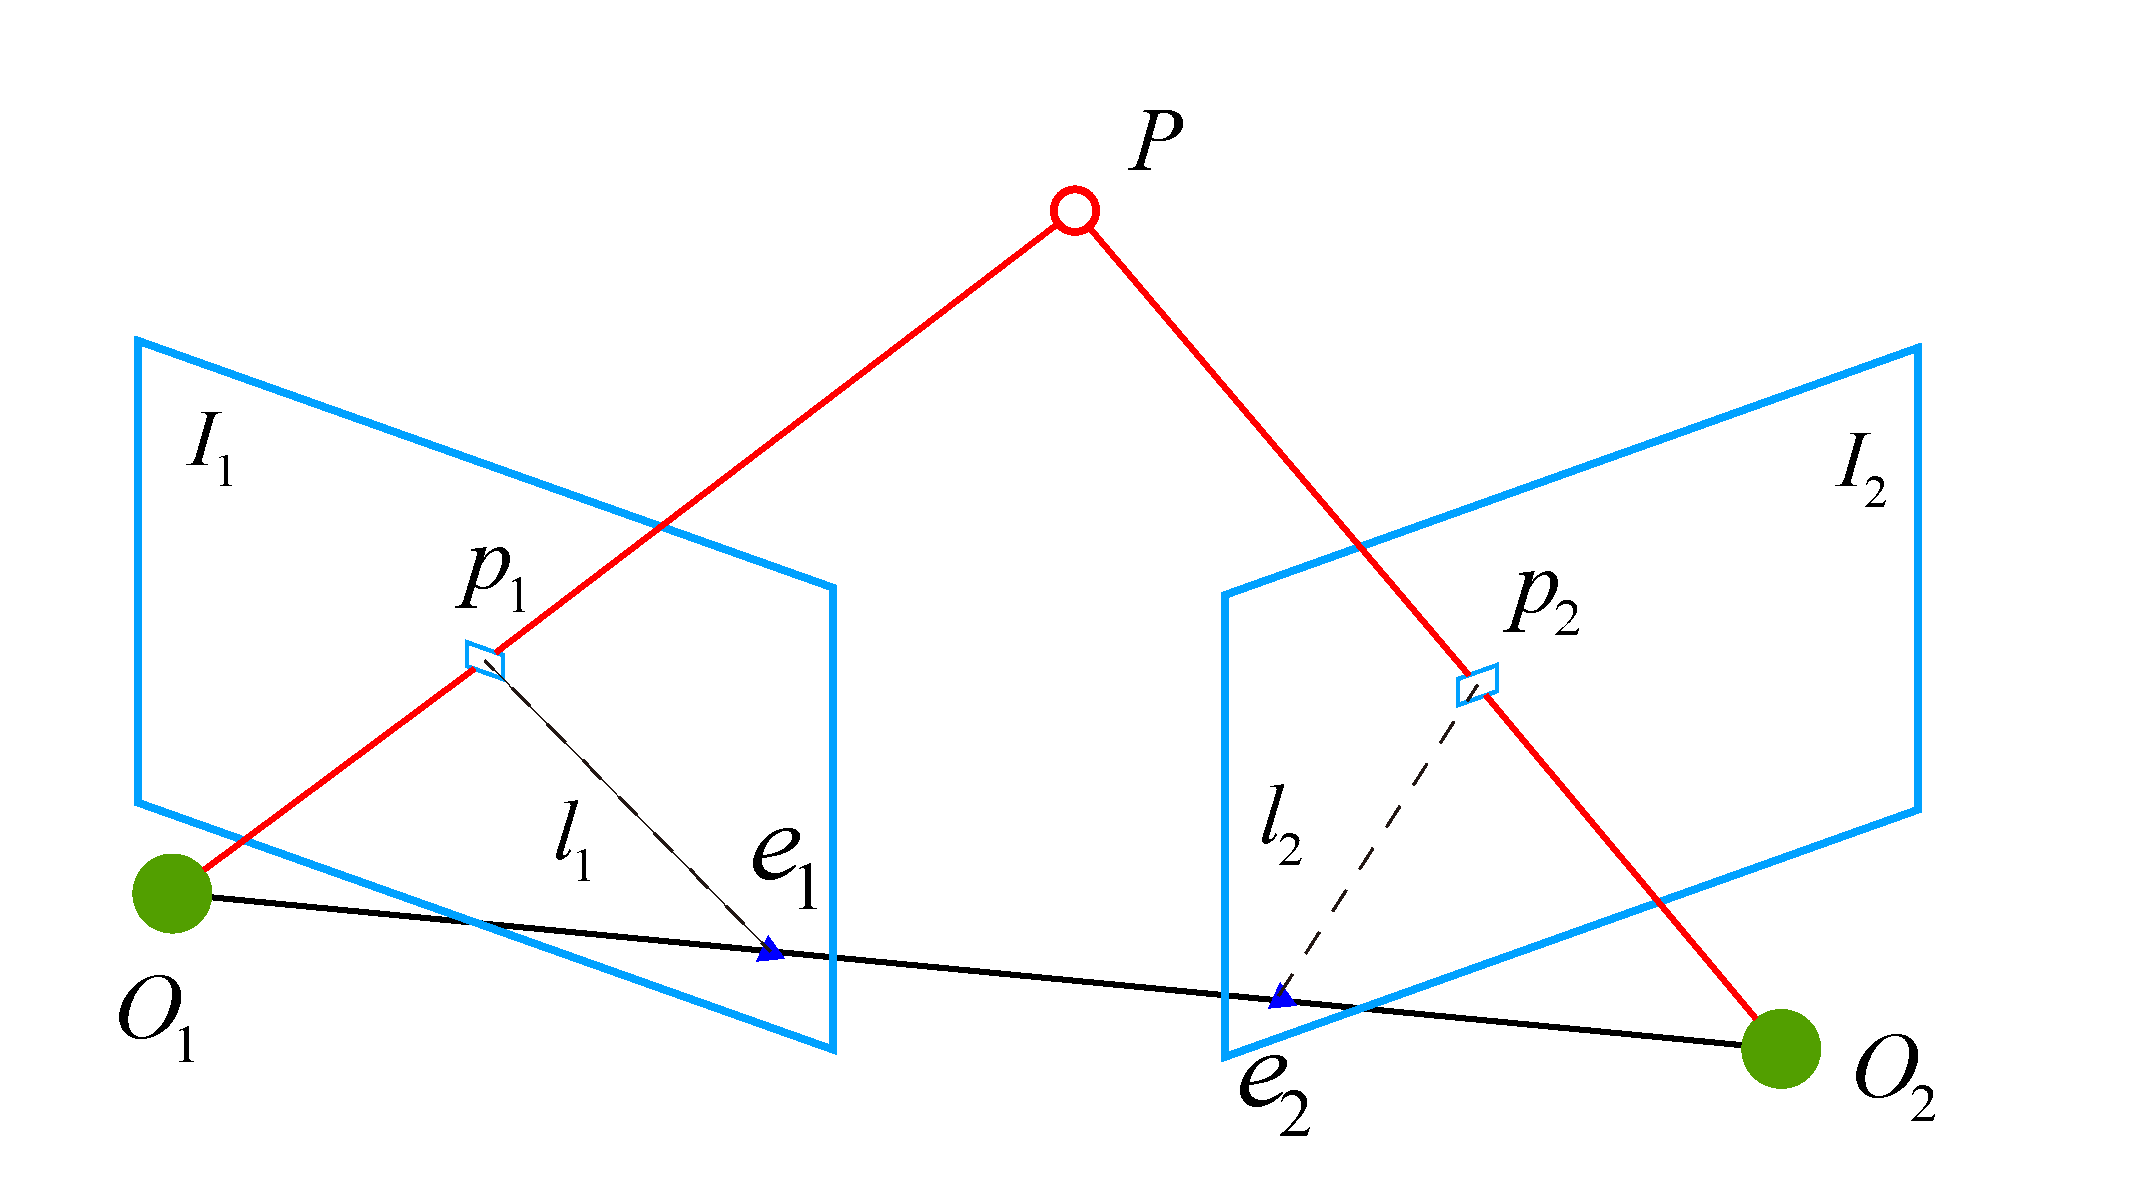
\includegraphics[width=0.6\linewidth]{vo1/fundamental}
	\caption{The epipolar constraints.}
	\label{fig:doubleview}
\end{figure}

Take \autoref{fig:doubleview}~ as an example. Our goal is to find the motion between two frames $I_{1}, I_{2}$. Define the motion from the first frame to the second frame as $\mathbf{R}, \mathbf{t}$, and the centers of the two cameras as $O_{1}, O_{2}$. Now, consider that there is a feature point $p_{1}$ in $I_{1}$, which corresponds to the feature point $p_{2}$ in $I_{2}$, obtained through feature matching. If the matching is correct, it means that they are indeed the projection of the same point. Now we need some terms to describe the geometric relationship between them. First, the line $\overrightarrow{O_{1}p_{1}}$ and the line $\overrightarrow{O_{2}p_{2}}$ will intersect at the point $P$ in the 3D space. The three points $O_{1}, O_{2}, and P$ can determine a plane, and it is called the epipolar plane. The intersection of the line of $O_{1}O_{2}$ and the image plane $I_{1}, I_{2}$ is $e_{1}, e_{2}$, respectively. The $e_{1}, e_{2}$ is called epipoles, and $O_{1}O_{2}$ is called the baseline. We call the intersecting line $l_{1},l_{2}$ between the polar plane and the two image planes $I_{1}, I_{2}$ as the epipolar line.

From the first frame, the ray $\overrightarrow{O_1 p_1}$ represents the possible spatial locations where a pixel may appear since all points on the ray will be projected to the same pixel. Meanwhile, suppose we don't know the location of $P$. When we look at the second image, the connection $\overrightarrow{e_2 p_2}$ (i.e., the epipolar line in the second image) is the possible projected positions of the point $P$, as well as the projection of the ray $\overrightarrow{O_1 p_1}$ in the second image. Now, since we have determined the pixel location of $p_2$ through feature matching, we can infer the spatial location of $P$ and the camera movement, as long as the feature matching is correct. If there is no feature matching, we can't determine where the $p_2$ is on the epipolar line. At that time, we must search on the epipolar line $l_2$ to get the correct match, which will be discussed in lecture~\ref{cpt:12}.

Now, let's look at the geometric relationship algebraically. Define the spatial position of $P$ in the first frame to be:
\[
\mathbf{P}=[X,Y,Z]^T.
\]
According to the pinhole camera model introduced in lecture~\ref{cpt:5}, we know that the pixel positions of the two pixels $\mathbf{p}_1,\mathbf{p}_2$ are:
\begin{equation}
\label{eq:7.1}
s_1 {\mathbf{p}_1} = \mathbf{KP},\quad s_2 \mathbf{p}_2 = \mathbf{K}\left( \mathbf{RP + t} \right),
\end{equation}
where $\mathbf{K}$ is the camera intrinsic  matrix, and $\mathbf{R}, \mathbf{t}$ are the camera motions between two frames. Specifically, they are $\mathbf{R}_{21}$ and $\mathbf{t}_{21}$, i.e. transformation from the first frame to the second. We can also write them in Lie algebra form.

Sometimes, we use homogeneous coordinates to represent pixels. When using homogeneous coordinates, a vector will be equal to itself multiplied by any non-zero constant. This is usually used to express a projection relationship. For example, $s_1 \mathbf{p}_1$ and $\mathbf{p}_1$ form a projection relationship, and they are equal in the sense of homogeneous coordinates. We call this equal \textit{up to a scale}, denoted as:
\begin{equation}
s\mathbf{p} \simeq \mathbf{p}.
\end{equation}
Then, the relationship between two projections can be written as:
\begin{equation}
 {\mathbf{p}_1} \simeq \mathbf{KP},\quad \mathbf{p}_2 \simeq \mathbf{K}\left( \mathbf{RP + t} \right).
\end{equation}

Now, let
\begin{equation}
{\mathbf{x}_1} = {\mathbf{K}^{ - 1}}{\mathbf{p}_1}, \quad {\mathbf{x}_2} = {\mathbf{K}^{ - 1}}{\mathbf{p}_2}.
\end{equation}

Here, $\mathbf{x}_1, \mathbf{x}_2$ are the coordinates on the normalized plane of two pixels. Substituting to the above equation, we get:
\begin{equation}
{\mathbf{x}_2} \simeq \mathbf{R} {\mathbf{x}_1} + \mathbf{t}.
\end{equation}

Left multiply both sides by $\mathbf{t}^\wedge$. Recalling the definition of $^\wedge$, this is equivalent to the outer product of both sides with $\mathbf{t}$:
\begin{equation}
\mathbf{t}^\wedge \mathbf{x}_2 \simeq \mathbf{t}^\wedge \mathbf{R} \mathbf{x}_1.
\end{equation}

Then, left multiply $\mathbf{x}_2^T$ on both sides:
\begin{equation}
\mathbf{x}_2^T \mathbf{t}^\wedge \mathbf{x}_2 \simeq \mathbf{x}_2^T \mathbf{t}^\wedge \mathbf{R} \mathbf{x}_1.
\end{equation}

On the left side, $\mathbf{t}^\wedge \mathbf{x}_2$ is a vector orthogonal to both $\mathbf{t}$ and $\mathbf{x}_2$. So its inner product with $\mathbf{x}_2$ will get 0. Since the left side of the equation is strictly zero, it is also zero after multiplying by any non-zero constant, so we can turn $\simeq$ back to the usual equal sign. Therefore, we have a concise equation:
\begin{equation}
\mathbf{x}_2^T \mathbf{t}^\wedge \mathbf{R} \mathbf{x}_1 = 0.
\end{equation}

Substituting the $\mathbf{p}_1, \mathbf{p}_2$ again, we have:
\begin{equation}
\mathbf{p}_2^T \mathbf{K}^{-\mathrm{T}} \mathbf{t}^\wedge \mathbf{R} \mathbf{K}^{-1} \mathbf{p}_1  = 0.
\end{equation}

Both equations are called \textbf{epipolar constraint}, which is famous for its conciseness. Geometrically, it means $O_1, P, O_2$ are coplanar. The epipolar constraint encodes both translation and rotation. We define two matrices: \textit{Fundamental} matrix $\mathbf{F}$ and \textit{essential} Matrix $\mathbf{E}$ from this equation: 
\begin{equation}
\mathbf{E} = \mathbf{t}^ \wedge \mathbf{R}, \quad \mathbf{F} = \mathbf{K}^{ -\mathrm{T}} \mathbf{E} {\mathbf{K}^{ - 1}}, \quad \mathbf{x}_2^T \mathbf{E} {\mathbf{x}_1} = \mathbf{p}_2^T \mathbf{F} {\mathbf{p}_1} = 0.
\end{equation}

The epipolar constraint gives the spatial relationship of two matching points concisely. Therefore, the camera pose estimation problem can be summarized as the following two steps:

\begin{enumerate}
	\item Find $\mathbf{E}$ or $\mathbf{F}$ based on the pixel positions of the matched points.
	\item Find $\mathbf{R}, \mathbf{t}$ based on $\mathbf{E}$ or $\mathbf{F}$.
\end{enumerate}

Since $\mathbf{E}$ and $\mathbf{F}$ only differ from the camera internal parameters, and the internal parameters are assumed to be known in SLAM problem \footnote{However, in SfM research, it may be unknown and need to be estimated. }, so the simpler form $\mathbf{E}$ is often used in practice. Let's take $\mathbf{E}$ as an example to introduce how to solve the above two problems.

\subsection{Essential Matrix}
By definition, the essential matrix $\mathbf{E} = \mathbf{t}^\wedge \mathbf{R}$. It is a matrix of $3\times 3$ with 9 unknown variables. So, can any matrix of the size $3 \times 3$ be an essential matrix? From the structure of $\mathbf{E}$, there are the following points worth noting:

\begin{itemize}
	\item The essential matrix is defined by the epipolar constraint. Since the epipolar constraint is the constraint of an\textit{ equal-to-zero }equation, after multiplying $\mathbf{E}$ by any non-zero constant, the constraint is still satisfied. We call this $\mathbf{E}$ 's equivalence under different scales.
	\item According to $\mathbf{E} = \mathbf{t}^ \wedge \mathbf{R}$, it can be proved that ~\cite{Hartley2003}, the singular value of the essential matrix $\mathbf{E}$ must be in the form of $[\sigma, \sigma, 0]^T$. This is called internal properties of essential matrix.
	\item On the other hand, since translation and rotation each have 3 degrees of freedom, $\mathbf{t}^\wedge \mathbf{R}$ has 6 degrees of freedom. But due to the equivalence of scales, $\mathbf{E}$ actually has 5 degrees of freedom.
\end{itemize}

The fact that $\mathbf{E}$ has 5 degrees of freedom indicates that we can use at least 5 pairs of points to solve $\mathbf{E}$. However, the internal property of $\mathbf{E}$ is nonlinear, which could cause trouble in the estimation. Therefore, it is also possible to consider only its scale equivalence and use 8 pairs of matched points to estimate $\mathbf{E}$. This is the classic \textit{eight-point-algorithm} {\cite{Hartley1997, Longuet-Higgins1987}}. The eight-point method only uses the linear properties of $\mathbf{E}$, so it can be solved under the framework of linear algebra. Let's take a look at how the eight-point method works.

Consider a pair of matched points, their normalized coordinates are $\mathbf{x}_{1}=[u_{1},v_{1},1]^T$, $\mathbf{x}_{2}=[u_{2},v_{2},1]^T$. According to the polar constraints, we have:
\begin{equation}
\begin{pmatrix} 
u_{2},v_{2},1
\end{pmatrix}
\begin{pmatrix}
 e_{1} & e_{2} & e_{3}\\ 
 e_{4} & e_{5} & e_{6}\\ 
 e_{7} & e_{8} & e_{9} 
\end{pmatrix}
\begin{pmatrix} 
u_{1}\\v_{1}\\1
\end{pmatrix}
=0.
\end{equation}

We rewrite the matrix $\mathbf{E}$ in the vector form:
\[
\mathbf{e}= [e_{1},e_{2},e_{3},e_{4},e_{5},e_{6},e_{7},e_{8},e_{9}]^T,
\]
Then the epipolar constraint can be written in a linear form related to $\mathbf{e}$:
\begin{equation}
[u_{2}u_{1},u_{2}v_{1},u_{2},v_{2}u_{1},v_{2}v_{1},v_{2},u_{1},v_{1},1] \cdot  \mathbf{e}=0.
\end{equation}

Analogously, we stack all the points into one equation and obtain a linear equation system (where $u^i, v^i$ represent the $i$-th feature point): 
\begin{equation}
\label{Eq:eight-point}
\begin{pmatrix}
u_{2}^{1}u_{1}^{1}& u_{2}^{1}v_{1}^{1}& u_{2}^{1}& v_{2}^{1}u_{1}^{1}& v_{2}^{1}v_{1}^{1}& v_{2}^{1} &u_{1}^{1} &v_{1}^{1}&1\\
u_{2}^{2}u_{1}^{2}& u_{2}^{2}v_{1}^{2}& u_{2}^{2}& v_{2}^{2}u_{1}^{2}& v_{2}^{2}v_{1}^{2}& v_{2}^{2} &u_{1}^{2} &v_{1}^{2}&1\\
\vdots & \vdots & \vdots & \vdots & \vdots & \vdots & \vdots & \vdots \\
u_{2}^{8}u_{1}^{8}& u_{2}^{8}v_{1}^{8}& u_{2}^{8}& v_{2}^{8}u_{1}^{8}& v_{2}^{8}v_{1}^{8}& v_{2}^{8} &u_{1}^{8}&v_{1}^{8}&1\\
\end{pmatrix}
\begin{pmatrix}
e_{1}\\ e_{2}\\ e_{3}\\  e_{4}\\ e_{5}\\ e_{6}\\ e_{7}\\ e_{8}\\ e_{9}  
\end{pmatrix}
=0.
\end{equation}


These eight equations form a linear equation system. Its coefficient matrix is composed of 2D feature point positions, and its size is $8 \times 9$. $\mathbf{e}$ is located in the null space of this matrix. If the coefficient matrix is of full rank (i.e., 8), then its null space dimension is 1, meaning that $\mathbf{e}$ forms a line. This is consistent with the scale equivalence of $\mathbf{e}$. If the matrix composed of 8 pairs of matching points meets the condition of rank 8, then the elements of $\mathbf{E}$ can be solved uniquely by the above equation.

The next question is how to recover the movement of the camera $\mathbf{R}, \mathbf{t}$ according to the estimated essential matrix $\mathbf{E}$. This process is obtained by singular value decomposition (SVD). Let the SVD decomposition of $\mathbf{E}$ be:
\begin{equation}
\mathbf{E} = \mathbf{U} \boldsymbol{\Sigma} \mathbf{V}^T,
\end{equation}
where $\mathbf{U}, \mathbf{V}$ are orthogonal matrices, and $\boldsymbol{\Sigma}$ is the  singular value matrice. According to the internal properties of $\mathbf{E}$, we know that $\boldsymbol{\Sigma} = \mathrm{diag}( \sigma, \sigma, 0 )$. In SVD decomposition, for any $\mathbf{E}$, there are two possible $\mathbf{t}, \mathbf{R}$:
\begin{equation}
\begin{array}{l}
\mathbf{t}_1^ \wedge  = \mathbf{U}{\mathbf{R}_Z}(\frac{\pi }{2}) \boldsymbol{\Sigma} {\mathbf{U}^T}, \quad {\mathbf{R}_1} = \mathbf{U} \mathbf{R}_Z^T(\frac{\pi }{2}){ \mathbf{V}^T}\\
\mathbf{t}_2^ \wedge  = \mathbf{U}{\mathbf{R}_Z}( - \frac{\pi }{2})\boldsymbol{\Sigma} {\mathbf{U}^T}, \quad  {\mathbf{R}_2} = \mathbf{U} \mathbf{R}_Z^T( - \frac{\pi }{2}){\mathbf{V}^T}.
\end{array}
\end{equation}

Among them, $\mathbf{R}_Z\left(\frac{\pi }{2}\right)$ represents the rotation matrix obtained by rotating $90^\circ$ along the $Z$ axis. Since $-\mathbf{E}$ is equivalent to $\mathbf{E}$, taking the minus sign for any $\mathbf{t}$ will also get the same result. Therefore, when decomposing from $\mathbf{E}$ to $\mathbf{t}, \mathbf{R}$, there are a total of \textbf{four} possible solutions.

\autoref{fig:epipolar-solution}~ shows the four solutions obtained by decomposing the essential matrix. We know the projection (red) of the space point on the camera (blue line) and want to solve the camera's motion. In the case of keeping the redpoint unchanged, four possible situations can be drawn. Fortunately, only in the first solution, $P$ has positive depths in both cameras. Therefore, we can substitute any points into the four solutions and check the depth's sign to determine which solution is correct.

\begin{figure}[!htp]
	\centering
	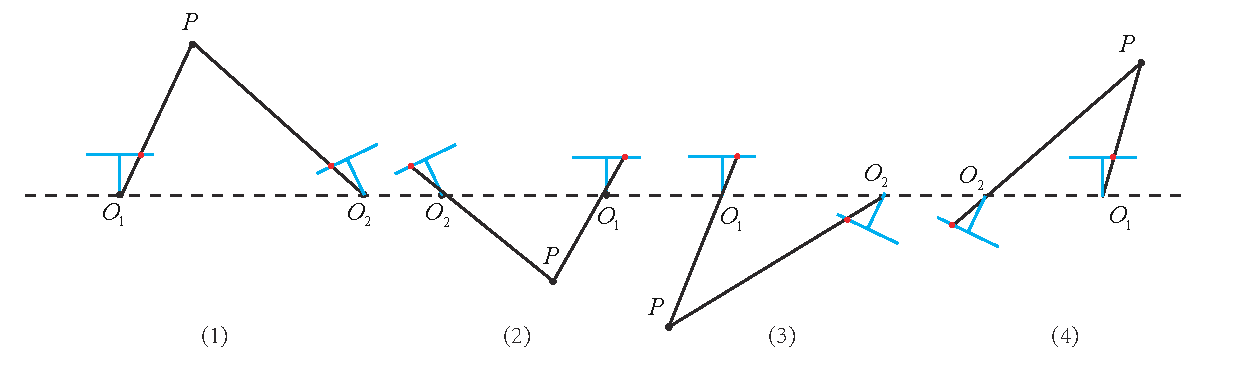
\includegraphics[width=1.0\linewidth]{vo1/epipolar-solution}
	\caption{We get four solutions when decomposing the essential matrix. }
	\label{fig:epipolar-solution}
\end{figure}

If we use the internal properties of $\mathbf{E}$, then it has only five degrees of freedom. So at least five pairs of matched points can be used to solve the camera motion {\cite{Li2006, Nister2004a}}. However, this approach is more complicated. Since there are usually dozens or even hundreds of matching points for engineering realization, it is often not helpful to reduce from 8 pairs to 5 pairs. To keep it simple, we only introduce the basic eight-point method here.

There is one remaining problem: $\mathbf{E}$ solved by linear equations may not satisfy the internal properties, i.e. its singular value is not necessarily in the form of ${\sigma}, {\sigma}, 0$. At this time, we will deliberately adjust the $\boldsymbol{\Sigma}$ matrix to look like the above. The usual procedure is to perform SVD decomposition on the $\mathbf{E}$ obtained by the eight-point method. Assume the singular value matrix is $\boldsymbol{\Sigma} = \mathrm{diag} (\sigma_1, \sigma_2, \sigma_3)$, and $\sigma_1 \geqslant \sigma_2 \geqslant \sigma_3$. We may take:
\begin{equation}
\mathbf{E} = \mathbf{U} \mathrm{diag} (\frac{\sigma_1+\sigma_2}{2}, \frac{\sigma_1+\sigma_2}{2}, 0) \mathbf{V}^T.
\end{equation}
This is equivalent to projecting the calculated essential matrix onto the manifold where $\mathbf{E}$ is located. A simpler approach is to take the singular value matrix as $\mathrm{diag} (1,1,0)$, due to $\mathbf{E}$'s scale equivalence, so it is also reasonable.

\subsection{Homography}
In addition to the fundamental matrix and the essential matrix, there is another common matrix in two-view geometry: the homography matrix $\mathbf{H}$, which describes the mapping relationship between two planes. If the feature points in the scene all fall on the same plane (such as walls, ground, etc.), we can estimate the motion through the homography matrix. This situation is more common in top-view cameras carried by drones or sweepers. 

The homography matrix usually describes the transformation between some points on a common plane between two images. Consider that there is a pair of matched feature points $p_{1}$ and $p_{2}$ in the images $I_{1}$ and $I_{2}$. These feature points fall on the plane $P$. Let this plane satisfy the equation of:
\begin{equation}
\mathbf{n}^T \mathbf{P} + d = 0.
\end{equation}
Rearrange it:
\begin{equation}
- \frac{\mathbf{n}^T \mathbf{P} }{d} = 1.
\end{equation}
Recalling \eqref{eq:7.1}, we have: 
\begin{align*}
\mathbf{p}_2 &\simeq \mathbf{K} ( \mathbf{R} \mathbf{P} + \mathbf{t} ) \\ 
&\simeq \mathbf{K} \left( \mathbf{R} \mathbf{P} + \mathbf{t} \cdot (- \frac{\mathbf{n}^T \mathbf{P} }{d}) \right) \\
&\simeq \mathbf{K} \left( \mathbf{R} - \frac{\mathbf{t} \mathbf{n}^T }{d} \right) \mathbf{P} \\ 
&\simeq \underbrace{\mathbf{K} \left( \mathbf{R} - \frac{\mathbf{t} \mathbf{n}^T }{d} \right) \mathbf{K}^{-1}}_{\mathbf{H}} \mathbf{p}_1.
\end{align*}

So, we get a direct description of the transformation between $\mathbf{p}_1$ and $\mathbf{p}_2$, denoting the middle part as $\mathbf{H}$, so:
\begin{equation}
\mathbf{p}_2 \simeq \mathbf{H} \mathbf{p}_1.
\end{equation}

Its definition is related to the parameters of rotation, translation, and plane coefficients. Similar to the fundamental matrix $\mathbf{F}$, the homography matrix $\mathbf{H}$ is also a matrix of $3 \times 3$. Solving this is similar to that of $\mathbf{F}$. Calculate $\mathbf{H}$ based on the matching points, and then decompose it to find rotation and translation. Expand the above formula, get:
\begin{equation}
\begin{pmatrix} 
u_{2}\\v_{2}\\1
\end{pmatrix}
\simeq
\begin{pmatrix}
 h_{1} & h_{2} & h_{3}\\ 
 h_{4} & h_{5} & h_{6}\\ 
 h_{7} & h_{8} & h_{9} 
\end{pmatrix}
\begin{pmatrix} 
u_{1}\\v_{1}\\1
\end{pmatrix}.
\end{equation}

Note that the equal sign here is still $\simeq$, not the ordinary equal sign, so the $\mathbf{H}$ matrix can also be multiplied by any non-zero constant. We can make $h_9 = 1$ in practice (when it takes a non-zero value). Then according to the third row, remove this non-zero factor. So we have:
\[
\begin{aligned}
u_{2}&=\frac{h_{1}u_{1}+h_{2}v_{1}+h_{3}}{h_{7}u_{1}+h_{8}v_{1}+h_{9}}\\
v_{2}&=\frac{h_{4}u_{1}+h_{5}v_{1}+h_{6}}{h_{7}u_{1}+h_{8}v_{1}+h_{9}}.
\end{aligned}
\]
Rearrange it:
\[
\begin{gathered}
h_{1}u_{1}+h_{2}v_{1}+h_{3}-h_{7}u_{1}u_{2}-h_{8}v_{1}u_{2}=u_{2}\\
h_{4}u_{1}+h_{5}v_{1}+h_{6}-h_{7}u_{1}v_{2}-h_{8}v_{1}v_{2}=v_{2}.
\end{gathered}
\]

A pair of matching points can construct two constraints, so the homography matrix with 8 degrees of freedom can be estimated by 4 pairs of matched features \footnote{In fact, there are three constraints, but the third one is linear dependent on the former two, so only the first two are taken.} (in the case of non-degenerate, which means these feature points cannot have three collinear points).  We solve the following linear equations to compute the $\mathbf{H}$: (when $h_9 = 0$, the right side is zero):
\begin{equation}
\begin{pmatrix}
u_{1}^{1}& v_{1}^{1}& 1 & 0 & 0 & 0 & -u_{1}^{1}u_{2}^{1} & -v_{1}^{1}u_{2}^{1}\\
0 & 0 & 0& u_{1}^{1}& v_{1}^{1}& 1 &  -u_{1}^{1}v_{2}^{1} & -v_{1}^{1}v_{2}^{1}\\
u_{1}^{2}& v_{1}^{2}& 1 & 0 & 0 & 0 & -u_{1}^{2}u_{2}^{2} & -v_{1}^{2}u_{2}^{2}\\
0 & 0 & 0& u_{1}^{2}& v_{1}^{2}& 1 &  -u_{1}^{2}v_{2}^{2} & -v_{1}^{2}v_{2}^{2}\\
u_{1}^{3}& v_{1}^{3}& 1 & 0 & 0 & 0 & -u_{1}^{3}u_{2}^{3} & -v_{1}^{3}u_{2}^{3}\\
0 & 0 & 0& u_{1}^{3}& v_{1}^{3}& 1 &  -u_{1}^{3}v_{2}^{3} & -v_{1}^{3}v_{2}^{3}\\
u_{1}^{4}& v_{1}^{4}& 1 & 0 & 0 & 0 & -u_{1}^{4}u_{2}^{4} & -v_{1}^{4}u_{2}^{4}\\
0 & 0 & 0& u_{1}^{4}& v_{1}^{4}& 1 &  -u_{1}^{4}v_{2}^{4} & -v_{1}^{4}v_{2}^{4}
\end{pmatrix}
\begin{pmatrix}
 h_{1}\\h_{2}\\h_{3}\\ h_{4}\\h_{5}\\h_{6}\\ h_{7}\\h_{8}\\  
\end{pmatrix}
=
\begin{pmatrix}
u_{2}^{1}\\ v_{2}^{1}\\ u_{2}^{2}\\ v_{2}^{2}\\u_{2}^{3}\\ v_{2}^{3}\\u_{2}^{4}\\ v_{2}^{4}
\end{pmatrix}.
\end{equation}

This approach regards the $\mathbf{H}$ matrix as a vector and estimates the $\mathbf{H}$ by solving the linear equations, also known as the direct linear transform (DLT). Like the essential matrix, the homography matrix needs to be decomposed after to get the corresponding rotation matrix $\mathbf{R}$ and translation vector $\mathbf{t}$. The decomposition method includes numerical method  {\cite{faugeras1988motion, Zhang1996}} and analytical method  {\cite{malis2007deeper}}. Similar to the decomposition of the essential matrix, the decomposition of the homography matrix will also return four sets of rotation matrices and translation vectors as well as the plane coefficients. If the depths of the projected map points are all positive (in front of the camera), then two sets of solutions can be excluded. In the end, only two sets of solutions are left, and more prior information is needed to make a final decision. Usually, we can solve it by assuming the normal vector of the known scene plane. If the scene plane is parallel to the camera plane, then the theoretical value of the normal vector $\mathbf{n}$ is $\mathbf{1}^T$.

The homography is of great significance in SLAM. When the feature points are coplanar, or the camera motion is pure rotation, the degree of freedom of the fundamental matrix decreases, which causes degeneration. The real data is always noisy. If you stick to the eight-point method to solve the fundamental matrix, the fundamental matrix's redundant freedom will be mainly determined by the noise. To avoid the effects of degradation, we usually estimate the fundamental matrix $\mathbf{F}$ and the homography matrix $\mathbf{H}$ simultaneously and then choose one with the smaller reprojection error as the final result.

\section{Practice: Solving Camera Motion with Epipolar Constraints}
In the following section, let's solve the camera motion through the essential matrix. The program in the previous section provides feature matching results, and here we use them to calculate $\mathbf{E}$ or $\mathbf{F}$ and then decompose $\mathbf{E}$ to get $\mathbf{R}$ and $\mathbf{t}$. The whole program is solved using the algorithm provided by OpenCV. We encapsulate the feature extraction in the previous section into functions for later use. This section only shows the code for the pose estimation.

\begin{lstlisting}[language=c++,caption=slambook2/ch7/pose_estimation_2d2d.cpp (part)]
void pose_estimation_2d2d(std::vector<key point> key points_1,
    std::vector<key point> key points_2,
    std::vector<DMatch> matches,
    Mat &R, Mat &t) {
    // Camera Intrinsics,TUM Freiburg2
    Mat K = (Mat_<double>(3, 3) << 520.9, 0, 325.1, 0, 521.0, 249.7, 0, 0, 1);
    
    //-- Convert the matching point to the form of vector<Point2f>
    vector<Point2f> points1;
    vector<Point2f> points2;
    
    for (int i = 0; i < (int) matches.size(); i++) {
        points1.push_back(key points_1[matches[i].queryIdx].pt);
        points2.push_back(key points_2[matches[i].trainIdx].pt);
    }
    
    //-- Calculate fundamental matrix
    Mat fundamental_matrix;
    fundamental_matrix = findFundamentalMat(points1, points2, CV_FM_8POINT);
    cout << "fundamental_matrix is " << endl << fundamental_matrix << endl;
    
    //-- Calculate essential matrix
    Point2d principal_point(325.1, 249.7);  // camera principal point, calibrated in TUM dataset
    double focal_length = 521;      // camera focal length, calibrated in TUM dataset
    Mat essential_matrix;
    essential_matrix = findEssentialMat(points1, points2, focal_length, principal_point);
    cout << "essential_matrix is " << endl << essential_matrix << endl;
    
    //-- Calculate homography matrix
    //-- But the scene is not planar, and calculating the homography matrix here is of little significance
    Mat homography_matrix;
    homography_matrix = findHomography(points1, points2, RANSAC, 3);
    cout << "homography_matrix is " << endl << homography_matrix << endl;
    
    //-- Recover rotation and translation from the essential matrix.
    recoverPose(essential_matrix, points1, points2, R, t, focal_length, principal_point);
    cout << "R is " << endl << R << endl;
    cout << "t is " << endl << t << endl;
}
\end{lstlisting}

This function shows how to solve the camera motion from the 2D feature points. Then, we call it in the main function to get the camera motion:
\begin{lstlisting}[language=c++,caption=slambook2/ch7/pose_estimation_2d2d.cpp (part)]
int main( int argc, char** argv ){
    if (argc != 3) {
        cout << "usage: pose_estimation_2d2d img1 img2" << endl;
        return 1;
    }
    //-- Fetch images
    Mat img_1 = imread(argv[1], CV_LOAD_IMAGE_COLOR);
    Mat img_2 = imread(argv[2], CV_LOAD_IMAGE_COLOR);
    assert(img_1.data && img_2.data && "Can not load images!");
    
    vector<key point> key points_1, key points_2;
    vector<DMatch> matches;
    find_feature_matches(img_1, img_2, key points_1, key points_2, matches);
    cout << "In total, we get " << matches.size() << " set of feature points" << endl;
    
    //-- Estimate the motion between two frames
    Mat R, t;
    pose_estimation_2d2d(key points_1, key points_2, matches, R, t);
    
    //-- Check E=t^R*scale
    Mat t_x =
        (Mat_<double>(3, 3) << 0, -t.at<double>(2, 0), t.at<double>(1, 0),
        t.at<double>(2, 0), 0, -t.at<double>(0, 0),
        -t.at<double>(1, 0), t.at<double>(0, 0), 0);
    cout << "t^R=" << endl << t_x * R << endl;
    
    //-- Check epipolar constraints
    Mat K = (Mat_<double>(3, 3) << 520.9, 0, 325.1, 0, 521.0, 249.7, 0, 0, 1);
    for (DMatch m: matches) {
        Point2d pt1 = pixel2cam(key points_1[m.queryIdx].pt, K);
        Mat y1 = (Mat_<double>(3, 1) << pt1.x, pt1.y, 1);
        Point2d pt2 = pixel2cam(key points_2[m.trainIdx].pt, K);
        Mat y2 = (Mat_<double>(3, 1) << pt2.x, pt2.y, 1);
        Mat d = y2.t() * t_x * R * y1;
        cout << "epipolar constraint = " << d << endl;
    }
    return 0;
}
\end{lstlisting}

We get the values of $\mathbf{E}, \mathbf{F}$ and $\mathbf{H}$ in the function, and then verify whether the epipolar constraint is satisfied, and $\mathbf{t}^ \wedge \mathbf{R}$ and $\mathbf{E}$ are equivalent to non-zero numbers. Now, execute this program to see the output result:
\begin{lstlisting}[language=sh,caption=Terminal Input:]
% build/pose_estimation_2d2d 1.png 2.png
-- Max dist : 95.000000 
-- Min dist : 4.000000 
In total, we get 79 set of feature points
fundamental_matrix is 
[4.844484382466111e-06, 0.0001222601840188731, -0.01786737827487386;
-0.0001174326832719333, 2.122888800459598e-05, -0.01775877156212593;
0.01799658210895528, 0.008143605989020664, 1]
essential_matrix is 
[-0.0203618550523477, -0.4007110038118445, -0.03324074249824097;
0.3939270778216369, -0.03506401846698079, 0.5857110303721015;
-0.006788487241438284, -0.5815434272915686, -0.01438258684486258]
homography_matrix is 
[0.9497129583105288, -0.143556453147626, 31.20121878625771;
0.04154536627445031, 0.9715568969832015, 5.306887618807696;
-2.81813676978796e-05, 4.353702039810921e-05, 1]
R is 
[0.9985961798781875, -0.05169917220143662, 0.01152671359827873;
0.05139607508976055, 0.9983603445075083, 0.02520051547522442;
-0.01281065954813571, -0.02457271064688495, 0.9996159607036126]
t is 
[-0.8220841067933337;
-0.03269742706405412;
0.5684264241053522]

t^R=
[0.02879601157010516, 0.5666909361828478, 0.04700950886436416;
-0.5570970160413605, 0.0495880104673049, -0.8283204827837456;
0.009600370724838804, 0.8224266019846683, 0.02034004937801349]
epipolar constraint = [0.002528128704106625]
epipolar constraint = [-0.001663727901710724]
epipolar constraint = [-0.0008009088410884102]
......
\end{lstlisting}

It can be seen from the program's output that the accuracy of the epipolar constraints is around the order of $10 ^{-3}$. According to the previous discussion, there are 4 possibilities for $\mathbf{R}, \mathbf{t}$ obtained by decomposition. In this program, OpenCV will use triangulation to detect whether the detected point's depth is positive to select the correct solution.

\subsection*{Discussion}
From the demo, we can see that the result $\mathbf{E}$ and $\mathbf{F}$ are different by a camera intrinsic matrix. Although it is not numerically intuitive, their mathematical relationship can be verified by the program. Motion can be decomposed from $\mathbf{E}, \mathbf{F}$ and $\mathbf{H}$, but $\mathbf{H}$ needs to assume that the feature points are on the same plane. For this experiment's data, this assumption is not true, so we mainly use $\mathbf{E}$ to find the motion.

It is worth mentioning that since $\mathbf{E}$ itself has scale equivalence, the $\mathbf{t}, \mathbf{R}$ also have scale equivalence. And $\mathbf{R} \in \mathrm{SO}(3)$ has its own constraints, so we think that $\mathbf{t}$ has a \textbf{scale}. In other words, in the decomposition process, if $\mathbf{t}$ is multiplied by any non-zero constant, the decomposition is still valid. Therefore, we usually normalize $\mathbf{t}$ to make its length equal to 1.

\subsubsection{Scale Ambiguity}
The normalization of $\mathbf{t}$ directly leads to \textit{scale ambiguity in monocular vision}. For example, the first dimension of $\mathbf{t}$ output in the program is about 0.822. We are unsure that it refers to 0.822 meters or 0.822 centimeters. Because after multiplying $\mathbf{t}$ by any constant, the epipolar constraint is still valid. In other words, in monocular SLAM, the trajectory and map are simultaneously zoomed at any multiple, and the image we get is still the same. This has already been introduced in chapter~\ref{cpt:2}.

In the monocular vision, the normalization of $\mathbf{t}$ for two images is equivalent to fixing the scale. Although we don't know its real length, we use this $\mathbf{t}$ as unit 1 to calculate the camera motion and the 3D position of the feature points. This is called the initialization phrase of monocular SLAM. After initialization, 3D-2D can be used to calculate camera motion. The latter trajectory and map will use the fixed scale during initialization. Therefore, monocular SLAM has an inevitable initialization step. The two initialized images must have a certain amount of translation, and then the unit of trajectory and map will be determined by this translation.

In addition to normalizing $\mathbf{t}$, another method is to set the average depth of all the feature points during initialization to 1, or a fixed scale. Compared to set the length of $\mathbf{t}$ to 1, normalizing the depth of the feature points can control the scale of the scene and make the calculation more numerically stable. But there is no theoretical difference.

\subsubsection{The Problem of Pure Rotation}
In the decomposition of $\mathbf{E}$ to get $\mathbf{R}, \mathbf{t}$, if the camera is purely rotated, causing $\mathbf{t}$ to be zero, then $\mathbf{E}$ will also be zero, which will make it impossible for us to solve $\mathbf{R}$. However, we can rely on $\mathbf{H}$ to find the rotation at this time, but we cannot generally assume the scene is a plane. Also, in the rotation-only case, we cannot use triangulation to estimate the feature points' spatial position (this will be introduced later). So we can conclude that the monocular initialization cannot be performed in the pure rotation case. It must have a certain amount of translation. If there is no translation, the monocular SLAM system can not be initialized. In practice, if the translation is too small during initialization, it will also make the pose estimation and triangulation results unstable and even failed. In contrast, if the camera is moved left and right instead of rotating, it will be easy to initialize the monocular SLAM. Therefore, experienced SLAM researchers often choose to move the camera left and right to smoothly initialize in monocular SLAM, while novices tend to rotate the camera sitting in the seat. You can tell if one is really an experienced SLAM engineer or not from this.

\subsubsection{More Than Eight Pairs of Features}
When we get more than eight pairs of matched points (for example, we found 79 pairs of matches), we can calculate a least-square solution. Recalling the linearized epipolar constraint in \eqref{Eq:eight-point}, we denote the coefficient matrix on the left as $\mathbf{A}$:
\begin{equation}
\mathbf{A} \mathbf{e} = \mathbf{0} .
\end{equation}

For the eight-point method, the size of $\mathbf{A}$ is $8 \times 9$. If the given features are more than $8$, the equation constitutes an overdetermined equation, that is, $\mathbf{e}$ does not necessarily exist to make the above formula perfectly true. Therefore, it can be solved by minimizing in a quadratic form:
\begin{equation}
\mathop {\min }\limits_{\mathbf{e}} \left\| \mathbf{Ae} \right\|_2^2 = \mathop {\min }\limits_{\mathbf{e}} { \mathbf{e}^T} {\mathbf{A}^T} \mathbf{Ae}.
\end{equation}

So the $\mathbf{E}$ matrix in the sense of least-squares is obtained. However, we prefer to use random sample consensus (RANSAC) instead of least-squares to solve the above problem due to potential mismatches. RANSAC is general, applicable to many cases with incorrect data, and can handle data with incorrect matching.

\section{Triangulation}
\label{sec:7.5}
In the previous two sections, we introduced using the epipolar constraint to estimate the camera motion and discussed its limitations. After estimating the motion, the next step is to use the camera motion to estimate the spatial positions of the feature points. In monocular SLAM, the depths of the pixels cannot be obtained by a single image. We need to estimate the depths of the map points by the method of triangulation, shown in \autoref{fig:triangluar}.

\begin{figure}[!ht]
	\centering
	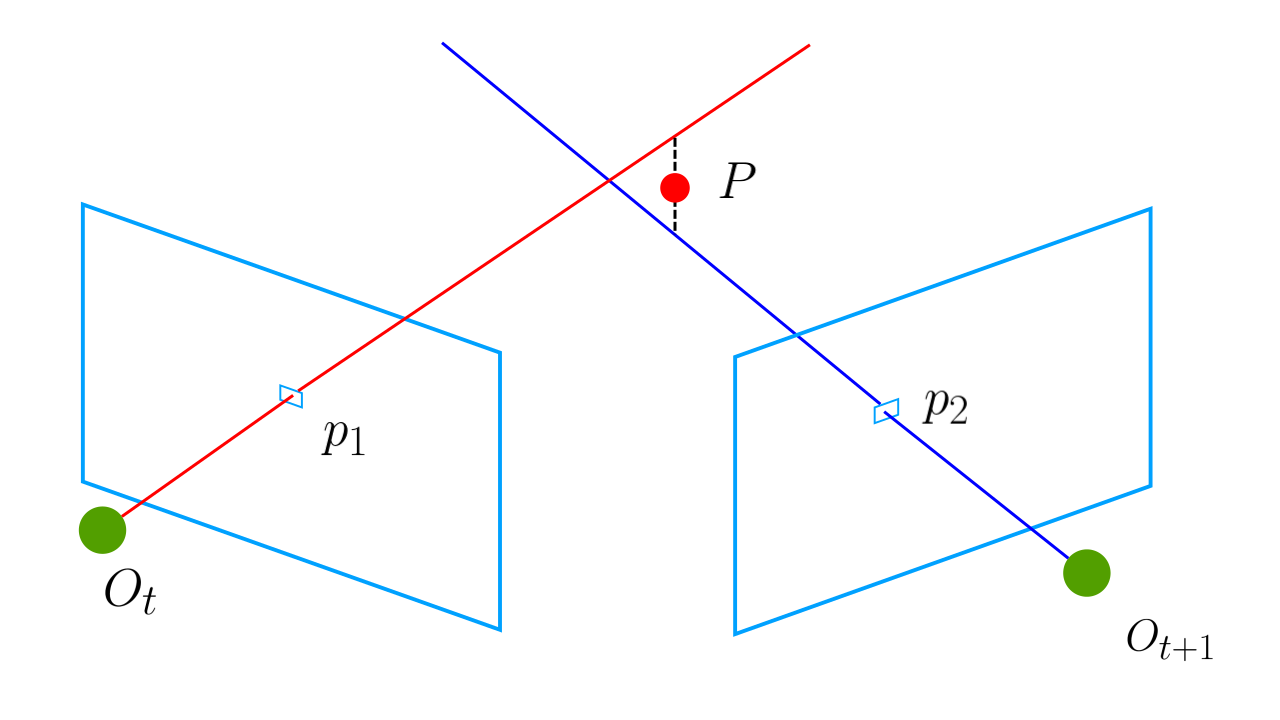
\includegraphics[width=0.9\linewidth]{vo1/triangularization}
	\caption{Use triangulation to estimate the depth.}
	\label{fig:triangluar}
\end{figure}

Triangulation refers to observing the same landmark point at different locations and determining the distance of the landmark point from the observed locations. Triangulation was first proposed by Gauss and used in metrology. It can also be applied to astronomy and geography. For example, we can estimate the distance to us from the angle of the star observed in different seasons. In SLAM, we mainly use triangulation to estimate the distance of pixels.

Similar to the previous section, consider the images $I_{1}$ and $I_{2}$, with the left image as a reference. The transform matrix to the right image is $\mathbf{T}$. The principal points of the camera are $O_{1}$ and $O_{2}$. The feature $p_{1}$ is in $I_{1}$, which corresponds to a feature $p_{2}$ in $I_{2}$. In theory, the straight line $O_{1}p_{1}$ and $O_{2}p_{2}$ will intersect at a point $P$ in the scene, which is the 3D map point. However, due to the noise, these two lines often fail to exactly intersect. Therefore, it can be solved in the sense of least-square.

According to the definition in epipolar geometry, let $\mathbf{x}_1, \mathbf{x}_2$ be the normalized coordinates of two feature points, then they satisfy:
\begin{equation}
s_2 \mathbf{x}_2 = s_1  \mathbf{R} \mathbf{x}_1 + \mathbf{t}.  
\end{equation}

Now we know the $\mathbf{R}$ and $\mathbf{t}$, we want to find the depth $s_1$ and $s_2$ of two feature points. Geometrically, you can find a 3D point on the ray $O_1 p_1$ to make its projection close to $\mathbf{p}_2$. Similarly, you can also find it on $O_2 p_2$ or in the middle of two lines. Different strategies correspond to different calculation methods, but the results are similar. For example, if we want to calculate $s_1$, we first multiply both sides of the above formula by $\mathbf{x}_2^\wedge$ to get:
\begin{equation}
\label{eq:x1tox2}
s_2 \mathbf{x}_2^\wedge \mathbf{x}_2 = 0 = s_1 \mathbf{x}_2^\wedge \mathbf{R} \mathbf{x}_1 + \mathbf{x}_2^\wedge \mathbf{t}. 
\end{equation}

The left side of this equation is zero, and the right side can be regarded as an equation of $s_1$, and $s_1$ can be obtained directly from it. With $s_1$, $s_2$ is also very easy to calculate. Thus, we get the depth of the points under the two frames and determine their spatial coordinates. Definitely, due to the existence of noise, our estimated $\mathbf{R}, \mathbf{t}$ may not exactly make the equation \eqref{eq:x1tox2} zero, so a more common approach is to find the least-square solution rather than a direct solution.

\section{Practice: Triangulation}
\subsection{Triangulation with OpenCV}
We demonstrate how to obtain the feature point's spatial position in the previous section through triangulation based on the camera pose solved by epipolar geometry. We will use the triangulation function provided by OpenCV here.

\begin{lstlisting}[language=c++,caption=slambook2/ch7/triangulation.cpp (part)]
void triangulation(
	const vector<key point> &key point_1,
	const vector<key point> &key point_2,
	const std::vector<DMatch> &matches,
	const Mat &R, const Mat &t,
	vector<Point3d> &points) {
	Mat T1 = (Mat_<float>(3, 4) <<
		1, 0, 0, 0,
		0, 1, 0, 0,
		0, 0, 1, 0);
	Mat T2 = (Mat_<float>(3, 4) <<
		R.at<double>(0, 0), R.at<double>(0, 1), R.at<double>(0, 2), t.at<double>(0, 0),
		R.at<double>(1, 0), R.at<double>(1, 1), R.at<double>(1, 2), t.at<double>(1, 0),
		R.at<double>(2, 0), R.at<double>(2, 1), R.at<double>(2, 2), t.at<double>(2, 0)
	);
	
	Mat K = (Mat_<double>(3, 3) << 520.9, 0, 325.1, 0, 521.0, 249.7, 0, 0, 1);
	vector<Point2f> pts_1, pts_2;
	for (DMatch m:matches) {
		// Convert pixel coordinates to camera coordinates
		pts_1.push_back(pixel2cam(key point_1[m.queryIdx].pt, K));
		pts_2.push_back(pixel2cam(key point_2[m.trainIdx].pt, K));
	}
	
	Mat pts_4d;
	cv::triangulatePoints(T1, T2, pts_1, pts_2, pts_4d);
	
	// Convert to non-homogeneous coordinates
	for (int i = 0; i < pts_4d.cols; i++) {
		Mat x = pts_4d.col(i);
		x /= x.at<float>(3, 0); // 归一化
		Point3d p(
			x.at<float>(0, 0),
			x.at<float>(1, 0),
			x.at<float>(2, 0)
		);
		points.push_back(p);
	}
}
\end{lstlisting}

Meanwhile, we can add the triangulation part to the main function and then draw each point's depth. Readers can run this program to view the triangulation results.

\subsection{Discussion}
Regarding triangulation, there is one more thing that must be noted.

Triangulation is caused by the \textit{translation}. Only when there is enough amount of translation, triangles in the epipolar geometry can be formed, and then the triangulation can be implemented. Therefore, triangulation cannot be used for pure rotation because the triangle does not exist in this case. Definitely, the real data is often not wholly equal to zero. In the presence of translation, we should also concern about the uncertainty of triangulation, which will lead to the triangulation contradiction.

As shown in \autoref{fig:triangulation-discuss}~, when the translation is small, the pixel's uncertainty will result in a more enormous depth uncertainty. That is to say, if the feature point moves by one pixel $\delta x$, the sight angle changes by an angle $\delta \theta$, then the measured depth will experience a difference of $\delta d$. It can be seen from the geometric relationship that when $\mathbf{t}$ is larger, $\delta d$ will be significantly smaller, meaning that when the translation is larger, the triangulation measurement will be more accurate at the same camera resolution. The quantitative analysis of the process can be proceeded by using the law of sine.

Therefore, to improve the accuracy of triangulation, one is to improve the accuracy of feature points extraction, which means to increase the image resolution, but this will cause the image to become larger and increase the computational cost. Another way is to increase the amount of translation. However, this will cause obvious changes in the image's appearance. For example, the box's side view initially blocked may be exposed, the lighting of the object changes, etc. Changes in appearance will make feature extraction and matching more difficult. In a nutshell, increasing the translation may lead to failure of matching; and if the translation is too small, the triangulation's accuracy is insufficient. This is the contradiction of triangulation. 

\begin{figure}[!ht]
	\centering
	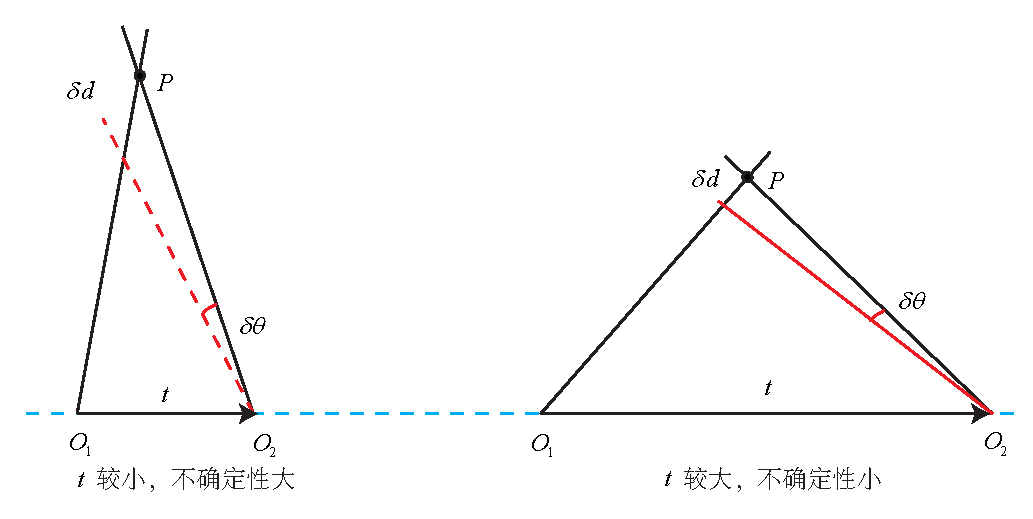
\includegraphics[width=1.0\linewidth]{vo1/triangulation-discuss.pdf}
	\caption{The contradiction of triangulation.}
	\label{fig:triangulation-discuss}
\end{figure}

In the monocular vision, since the image has no depth information, we have to wait for the feature points to be tracked for a few frames and then use triangulation to determine the new feature points' depth. This is also called delayed triangulation  {\cite{Davison2003}}. However, if the camera rotates in place, causing the parallax to be small, it is difficult to estimate the newly observed feature points' depth. This situation is common in robotics, as rotation is also a standard command for robots. In this case, monocular vision may suffer from tracking failures and incorrect scales.

Although this section only introduces the depth estimation of triangulation, we can also quantitatively calculate each feature point's location and uncertainty. Therefore, if we assume that the feature point obeys the Gaussian distribution and continuously observes it with the correct information, we can expect its variance will continue to decrease and even converge. This can be referred to as the depth filter. However, since its principle is more complicated, we will discuss it in later chapters~\ref{cpt:12}. Next, we will discuss the estimation of camera motion from 3D-2D matching points and 3D-3D estimation methods.

\section{3D−2D:PnP}
PnP (Perspective-n-Point) is a method to solve 3D to 2D motion estimation. It describes how to estimate the camera's pose when the $n$ 3D space points and their projection positions are known. As mentioned earlier, the 2D-2D epipolar geometry method requires eight or more point pairs (take the eight-point method as an example), and there have problems with initialization, pure rotation, and scale. However, if the 3D position of one of the feature points in the two images is known, then we need at least three pairs (and at least one additional point to verify the result) to estimate the camera motion. The 3D position of the feature point can be determined by triangulation or the depth map of an RGB-D camera. Therefore, in binocular or RGB-D visual odometry, we can directly use PnP to estimate camera motion. While in the monocular case, initialization must be conducted before using PnP. The 3D-2D method does not require epipolar constraints and can obtain better motion estimation in a few matching points. It is the most important pose estimation method.

There are many ways to solve PnP problems, for example, P3P {\cite{GaoHouTangEtAl2003}}, direct linear transformation (DLT), EPnP (Efficient PnP) {\cite{LepetitMoreno-NoguerFua2008}}, UPnP {\cite{Penate-SanchezAndrade-CettoMoreno-Noguer2013}}, etc. In addition, nonlinear optimization can be used to construct a least-square problem and iteratively solve it, which is commonly called the bundle adjustment. Let's look at DLT first, and then we will explain the bundle adjustment approach.

\subsection{Direct Linear Transformation}
Consider such a problem: we know the 3D positions of a point set and their projections in the camera, now we want to find the camera's pose. This problem can be used to solve the camera pose when a given map and image are given. If the 3D point is regarded as a point in another camera coordinate system, it can also solve the two cameras' relative motion problem. We will start with simple questions.

Consider a 3D spatial point $P$, its homogeneous coordinates are ${\mathbf{P}}=(X,Y,Z,1)^T$. In the image $I_{1}$, it is projected to the feature point ${\mathbf{x}}_{1}=(u_{1},v_{1},1)^T$(expressed as the normalized homogeneous coordinates). At this time, the pose of the camera $\mathbf{R}, \mathbf{t}$ is unknown. Similar to the solution of the homography matrix, we define the $3\times 4$ augmented matrix $[\mathbf{R}|\mathbf{t}]$, encoding rotation and translation information \footnote{This is different from the transformation matrix $\mathbf{T}$ in $\mathrm{SE}(3)$. }. We will write its expanded form as follows:
\begin{equation}
s
\begin{pmatrix}
u_{1} \\ v_{1} \\ 1
\end{pmatrix}
= \underbrace{
\begin{pmatrix}
t_{1} & t_{2} & t_{3} & t_{4}\\ 
t_{5} & t_{6} & t_{7} & t_{8}\\ 
t_{9} & t_{10} & t_{11} & t_{12}
\end{pmatrix}}_{[\mathbf{R}|\mathbf{t}]}
\begin{pmatrix}
X \\ Y \\ Z \\ 1
\end{pmatrix}.
\end{equation}

Eliminate $s$ with the last row to get two constraints:
\[
u_{1}=\frac{t_{1}X+t_{2}Y+t_{3}Z+t_{4}}{t_{9}X+t_{10}Y+t_{11}Z+t_{12}},\quad
v_{1}=\frac{t_{5}X+t_{6}Y+t_{7}Z+t_{8}}{t_{9}X+t_{10}Y+t_{11}Z+t_{12}}.
\]

To simplify the representation, define $\mathbf{T}$ as a row vector:
\[
\mathbf{t}_{1}=(t_{1},t_{2},t_{3},t_{4})^T,
\mathbf{t}_{2}=(t_{5},t_{6},t_{7},t_{8})^T,
\mathbf{t}_{3}=(t_{9},t_{10},t_{11},t_{12})^T.
\]

Now we have:
\[
\mathbf{t}_1^T\mathbf{P}-\mathbf{t}_3^T\mathbf{P} u_1=0,
\]
and
\[
\mathbf{t}_2^T\mathbf{P}-\mathbf{t}_3^T\mathbf{P} v_1=0.
\]

Please note that $\mathbf{t}$ is the variable to be determined. As you can see, each feature point provides two linear constraints on $\mathbf{t}$. Assuming there are a total of $N$ feature points, the following linear equations can be constructed:
\begin{equation}
\begin{pmatrix}
\mathbf{P}_{1}^T & 0 & -u_{1}\mathbf{P}_{1}^T	\\
0 & \mathbf{P}_{1}^T & -v_{1}\mathbf{P}_{1}^T	\\
\vdots & \vdots & \vdots			\\
\mathbf{P}_{N}^T & 0 & -u_{N}\mathbf{P}_{N}^T \\
0 & \mathbf{P}_{N}^T & -v_{N}\mathbf{P}_{N}^T
\end{pmatrix}
\begin{pmatrix}
\mathbf{t}_{1} \\ \mathbf{t}_{2} \\ \mathbf{t}_{3}
\end{pmatrix}
=0.
\end{equation}

Since $\mathbf{t}$ has a total dimension of 12, the linear solution of the matrix $\mathbf{T}$ can be achieved by at least six pairs of matching points. This method is called Direct Linear Transform (DLT). When the matching points are greater than 6 pairs, methods such as SVD can also be used to find the least-square solution of the overdetermined equation.

In the DLT solution, we directly regard the $\mathbf{T}$ matrix as 12 unknowns, ignoring the correlation between them. Because the rotation matrix $\mathbf{R} \in \mathrm{SO}(3)$, the solution obtained by DLT does not necessarily satisfy the $\mathrm{SE}(3)$ constraint. It is just a general matrix. The translation vector is easier to handle. It belongs to the vector space. For the rotation matrix $\mathbf{R}$, we must look for the best rotation matrix to approximate the matrix block of $3 \times 3$ on the left of $\mathbf{T}$ estimated by DLT. This can be done by QR decomposition  {\cite{Hartley2003, Chen1994}}, or it can be calculated like {\cite{Barfoot2016,Green1952}}:
\begin{equation}
\mathbf{R} \leftarrow {\left( {\mathbf{R}{\mathbf{R}^T}} \right)^{ - \frac{1}{2}}} \mathbf{R}.
\end{equation}
This can be seen as reprojecting the result from the matrix space onto the $\mathrm{SE}(3)$ manifold and converting it into two parts: rotation and translation.

What needs to be mentioned is that our $\mathbf{x}_1$ here uses normalized plane coordinates and neglects the influence of the intrinsic matrix $\mathbf{K}$. This is because $\mathbf{K}$ is usually assumed to be known in SLAM. Even if the intrinsic parameters are unknown, PnP can still be used to estimate the three quantities $\mathbf{K}, \mathbf{R}, \mathbf{t}$. However, due to the increase in the number of unknown variables, the result's quantity may be worse.

\subsection{P3P}
P3P is another way to solve PnP. It only uses 3 pairs of matching points and requires less data (this part refers to the~\cite{web:p3p}).

P3P requires establishing geometric relationships of the given 3 points. Its input data is 3 pairs of 3D-2D matching points. Define 3D points as $A, B, C$, 2D points as $a, b, c$, where the point represented by the lowercase letter is the projection of the point on the camera image plane represented by the corresponding uppercase letter, as shown in \autoref{fig:p3p}~. Also, P3P needs a pair of verification points to select the correct one from the possible solutions (similar to epipolar geometry). Denote the verification point pair as $D-d$ and the principal camera point as $O$. Suppose that $A, B, C$ are in the world coordinate frame, not the camera coordinate. Once the coordinates of the 3D point in the camera coordinate system can be calculated, we get the 3D−3D corresponding point and convert the PnP problem to the ICP problem.

\begin{figure}[!ht]
	\centering
	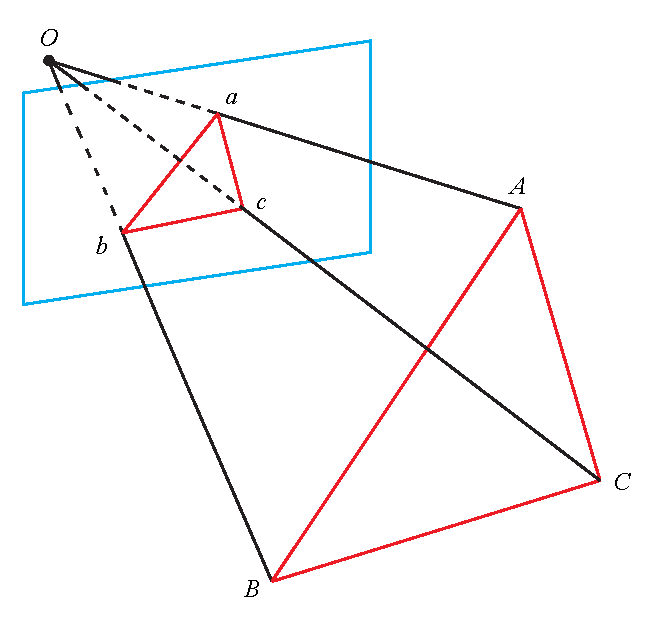
\includegraphics[width=0.54\linewidth]{vo1/p3p.pdf}
	\caption{The P3P problem.}
	\label{fig:p3p}
\end{figure}

Obviously, there is a relationship between triangles:
\begin{equation}
\Delta Oab - \Delta OAB, \quad \Delta Obc - \Delta OBC, \quad \Delta Oac - \Delta OAC.
\end{equation}

Consider the relationship between $Oab$ and $OAB$. Using the law of cosines, there are:
\begin{equation}
\overline{OA}^2 + \overline{OB}^2 - 2.\overline{OA}.\overline{OB}.\cos \left\langle a,b \right \rangle  = \overline{AB}^2.
\end{equation}

The other two triangles have similar properties, so we further get:
\begin{equation}
\begin{array}{l}
\overline{OA}^2 + \overline{OB}^2 - 2.\overline{OA}.\overline{OB}.\cos \left\langle a,b \right \rangle  = \overline{AB}^2\\
\overline{OB}^2 + \overline{OC}^2 - 2.\overline{OB}.\overline{OC}.\cos \left\langle b,c \right \rangle  = \overline{BC}^2\\
\overline{OA}^2 + \overline{OC}^2 - 2.\overline{OA}.\overline{OC}.\cos \left\langle a,c \right \rangle  = \overline{AC}^2.
\end{array}
\end{equation}

Divide all the above three equations by $\overline{OC}^2$ on both sides, and consider $x=\overline{OA}/\overline{OC},\ y=\overline{OB}/\overline{OC}$, we get:
\begin{equation}
\begin{array}{l}
{x^2} + {y^2} - 2.x.y.\cos \left\langle a,b \right \rangle  = \overline{AB}^2/\overline{OC}^2\\
{y^2} + {1^2} - 2.y.\cos \left\langle b,c \right \rangle  = \overline{BC}^2/\overline{OC}^2\\
{x^2} + {1^2} - 2.x.\cos \left\langle a,c \right \rangle  = \overline{AC}^2/\overline{OC}^2.
\end{array}
\end{equation}

Let $v = \overline{AB}^2/\overline{OC}^2,\ u.v = \overline{BC}^2/\overline{OC}^2,\ w.v = \overline{AC}^2/\overline{OC}^2$, then we have:
\begin{equation}
\begin{array}{l}
{x^2} + {y^2} - 2.x.y.\cos \left\langle a,b \right \rangle  - v = 0\\
{y^2} + {1^2} - 2.y.\cos \left\langle b,c \right \rangle  - u.v = 0\\
{x^2} + {1^2} - 2.x.\cos \left\langle a,c \right \rangle  - w.v = 0.
\end{array}
\end{equation}

Move $v$ in the first equation to the right side, and combine it with the other two equations, we have:
\begin{equation}
\begin{array}{l}
\left( {1 - u} \right){y^2} - u{x^2} - 2 \cos \left\langle b,c \right \rangle y + 2uxy\cos \left\langle a,b \right \rangle  + 1 = 0 \\
\left( {1 - w} \right){x^2} - w{y^2} - 2 \cos \left\langle a,c \right \rangle x + 2wxy\cos \left\langle a,b \right \rangle  + 1 = 0.
\end{array}
\end{equation}

Please distinguish the known from the unknown quantities in these equations. Since we know the positions of the 2D points in the image, the 3 cosine angles $\cos \left \langle a,b \right \rangle$, $\cos \left\langle b,c \right \rangle$, $\cos \left \langle a,c \right \rangle$ can be calculated. Meanwhile, $u=\overline{BC}^2/\overline{AB}^2, w=\overline{AC}^2/\overline{AB}^2$ can be calculated by the coordinates of $A, B, C$ in the world frame. Transforming to the camera frame does not change the ratio. The $x$ and $y$ are unknown and will change as the camera moves. Therefore, the equations are quadratic equations about two unknowns $x, y$. Analytically solving the equations is complicated and requires Wu's elimination method. It will not be introduced here. Interested readers could refer to the literature~\cite{GaoHouTangEtAl2003}. Analogous to the case of decomposing $\mathbf{E}$, this equation may get 4 solutions at most. Still, we can use the verification points to select the most probable solution and get the 3D of $A, B, C$ in the camera frame. Then, based on the 3D−3D point pair, the camera movement $\mathbf{R}, \mathbf{t}$ can be calculated, which will be introduced in section~\ref{sec:7.9}.

From the principle of P3P to solve PnP, we use the triangle relationships to solve the 3D coordinates of the projection points $a, b, c$ in the camera frame, and finally convert the problem into a 3D to 3D pose estimation problem. As we will see later, it is easy to solve the 3D-3D pose with matching information, so this idea is very effective. Some other methods, such as EPnP, also adopted this idea. However, P3P also has some deficiencies:

\begin{enumerate}
	\item P3P only includes the information of 3 points. When the given matched points are more than 3, it is difficult to use more information.
	\item If the 3D point or 2D point is affected by noise or a mismatch, the algorithm goes into trouble.
\end{enumerate}

People also proposed many other methods, such as EPnP, UPnP, and so on. They use more information and iteratively optimize the camera pose to eliminate noise as much as possible. However, compared to P3P, the principles are more complicated, so we recommend that readers read the original papers or understand the PnP process by practice. In SLAM, the usual approach is to first estimate the camera pose using P3P/EPnP and then construct a least-squares optimization problem to adjust the estimated values (bundle adjustment). When the camera motion is sufficiently continuous, or you can also assume that the camera does not move or move at a constant speed, you can use the estimated values as the initial values for optimization. Next, we look at the PnP problem from the perspective of nonlinear optimization.

\subsection{Solve PnP by Minimizing the Reprojection Error}
\label{sec:BA-vo1}
Other than the linear method, we can also construct the PnP problem as a nonlinear least-square problem about reprojection errors. This will use the knowledge from the chapters~\ref{cpt:4} and~\ref{cpt:5} of this book. The linear method mentioned above is often divided into many steps, such as estimating the camera pose first and then the point's position. While nonlinear optimization treats them as optimization variables and optimizes them together. This is a very general solution method. We can use it to optimize the results given by PnP or ICP. This type of problem, putting the camera and 3D points together to minimize, is generally referred to as bundle adjustment \footnote{The meaning of BA in different documents and contexts are not exactly the same. Some people only refer to problems that minimize the reprojection errors as BA, while others have a broader definition of BA. Even if the BA has only one camera, it can be called BA. I personally prefer the broader definition, so the method of calculating PnP here is also called BA.}.

We can build a bundle adjustment problem in PnP to optimize the camera pose. If the camera is moving continuously (as in most SLAM processes), we can also use BA directly to solve the camera pose. In this section, we will give the basic two-view form of this problem and then discuss the larger-scale BA problem in lecture~\ref{cpt:9}.

Suppose we have $n$ 3D space points $P$ and their projection $p$, we want to calculate the pose $\mathbf{R}, \mathbf{t}$ of the camera. Suppose the coordinates of a point are $\mathbf{P}_i=[X_i,Y_i,Z_i]^T$, and their projected pixel coordinates are $\mathbf{u}_i=[u_i,v_i]^ \mathrm{T}$. According to~\ref{cpt:5}, the relationship between the 2D pixel position and the 3D spatial position is:
\begin{equation}
s_i \left[ 
\begin{array}{l}
u_i \\ v_i \\ 1
\end{array}
\right] = \mathbf{K} \mathbf{T} \left[ 
\begin{array}{l}
X_i \\ Y_i \\ Z_i \\ 1
\end{array} \right]  .
\end{equation}
Or in the matrix form:
\[
{{s_i {\mathbf{u}}_i} = \mathbf{K} \mathbf{T} \mathbf{P}}_i.
\]

This equation includes a conversion from homogeneous coordinates to non-homogeneous coordinates implicitly. Or we can also use $\mathbf{R}\mathbf{P}+\mathbf{t}$. Now, due to the unknown camera pose and the noise of the observation points, there is a residual in the equation. Therefore, we sum up the residuals, construct a least-square problem, and then minimize it to find the most possible camera pose:
\begin{equation}
{\mathbf{T}^*} = \arg \mathop {\min }\limits_{\mathbf{T}}  \frac{1}{2}\sum\limits_{i = 1}^n {\left\| {{{\mathbf{u}}_i} - \frac{1}{s_i} \mathbf{K}\mathbf{T}{\mathbf{P}}_i} \right\|_2^2} .
\end{equation}

The residual term is the error of the projected position and the observed position, which is called the reprojection error. With homogeneous coordinates, this error has three dimensions. However, since the last dimension of ${\mathbf{u}}$ is 1, the error of this dimension is always zero, so we normally use non-homogeneous coordinates. Therefore, the error has only 2 dimensions. As shown in \autoref{fig:reprojection}~, we know that $p_1$ and $p_2$ are projections of the same space point $P$ through feature matching, but we don't know the pose of the camera. In the initial value, there is a certain distance between the projection of $P \hat{p}_2$ and the observed $p_2$. So we adjusted the pose of the camera to make this distance smaller. However, since this adjustment needs to consider many points, the goal is to reduce the overall error, and the error of each point usually can not be exactly zero.

\begin{figure}[!htp]
	\centering
	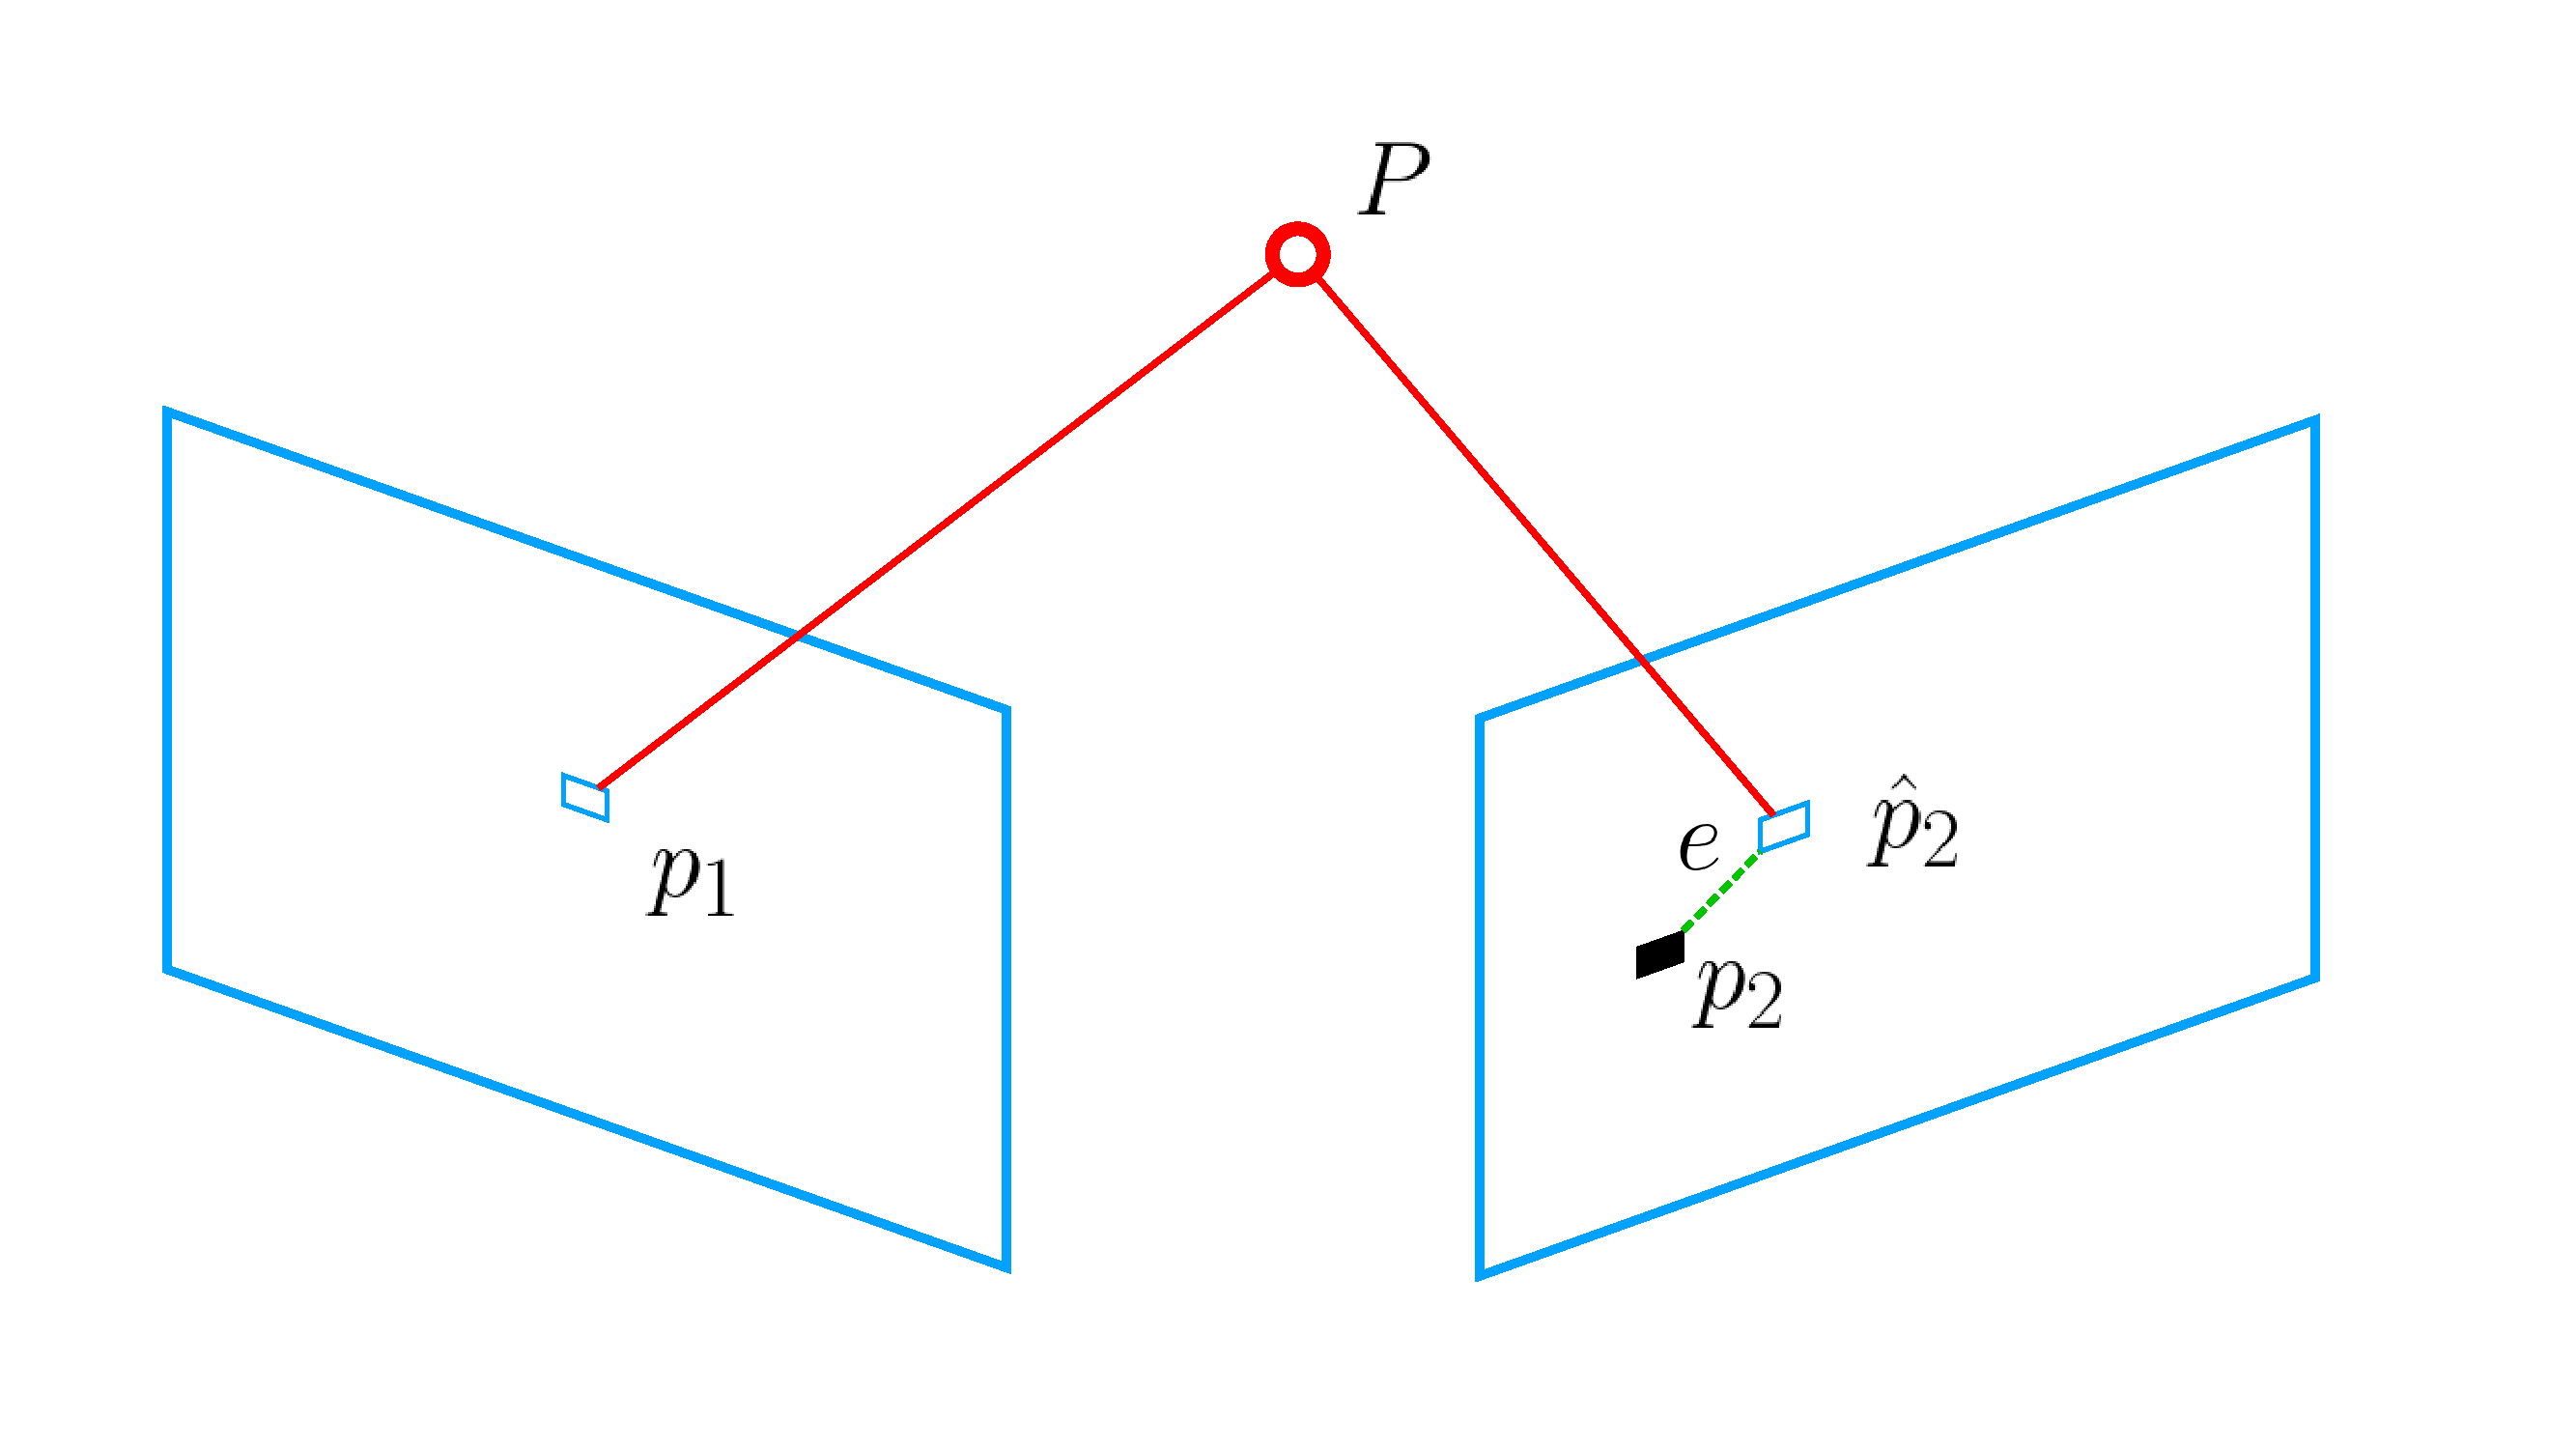
\includegraphics[width=0.8\linewidth]{vo1/reprojection}
	\caption{The reprojection error.}
	\label{fig:reprojection}
\end{figure}

We have already discussed the least-square optimization problem in chapter~\ref{cpt:6}. Using Lie algebra, we can construct an unconstrained optimization problem on the manifold, easily solved using optimization algorithms such as the Gauss-Newton method and Levenberg-Marquardt method. However, we need to calculate the derivative of each error term with respect to the optimization variable, which is also the linearization:
\begin{equation}
\mathbf{e}( \mathbf{x} + \Delta \mathbf{x} ) \approx \mathbf{e}(\mathbf{x}) + \mathbf{J} ^T\Delta \mathbf{x}.
\end{equation}

The form of $\mathbf{J}^T$ is worth discussing. Definitely, we can use numerical derivatives, but if we can derive an analytical form, we will prefer the analytical derivatives. Now, $\mathbf{e}$ is the pixel coordinate error (2-d) and $\mathbf{x}$ is the camera pose (6-d), $\mathbf{J}^T$ is a matrix of $2 \times 6$. Let's derive the form of $\mathbf{J}^T$.

We have introduced how to use the perturbation model to find the pose variable's derivative (chapter~\ref{cpt:4}). First, define the coordinates of the space point in the camera frame as $\mathbf{P}'$, and take out the first 3 dimensions:
\begin{equation}
\mathbf{P}' = \left( \mathbf{T}{\mathbf{P}} \right)_{1:3}= [X', Y', Z']^T.
\end{equation}

Then, the camera projection model with respect to $\mathbf{P}'$ is:
\begin{equation}
s {\mathbf{u}} = \mathbf{K} \mathbf{P}'.
\end{equation}

Expand it:
\begin{equation}
\left[ \begin{array}{l}
su\\
sv\\
s
\end{array} \right] = \left[ {\begin{array}{*{20}{c}}
	{{f_x}}&0&{{c_x}}\\
	0&{{f_y}}&{{c_y}}\\
	0&0&1
	\end{array}} \right]\left[ \begin{array}{l}
X'\\
Y'\\
Z'
\end{array} \right].
\end{equation}

Use the third row to eliminate $s$ (actually it is the distance of $\mathbf{P}'$), we get:
\begin{equation}
\label{eq:uv2xyz}
u = {f_x}\frac{{X'}}{{Z'}} + {c_x}, \quad v = {f_y}\frac{{Y'}}{{Z'}} + {c_y}.
\end{equation}

This is consistent with the camera model described in~\ref{cpt:5}. When we find the error, we can compare the $u, v$ here with the measured value to find the difference. After defining the intermediate variables, we left multiply $\mathbf{T}$ by a disturbance quantity $\delta \boldsymbol{\xi}$, and then consider the derivative of the change of $\mathbf{e}$ with respect to the disturbance quantity. Using the chain rule, it is:
\begin{equation}
\frac{{\partial \mathbf{e}}}{{\partial \delta \boldsymbol{\xi} }} = \mathop {\lim }\limits_{\delta \boldsymbol{\xi}  \to 0} \frac{{\mathbf{e}\left( {\delta \boldsymbol{\xi}  \oplus \boldsymbol{\xi} } \right)-\mathbf{e}(\boldsymbol{\xi})}}{{\delta \boldsymbol{\xi} }}  = \frac{{\partial \mathbf{e}}}{{\partial \mathbf{P}'}}\frac{{\partial \mathbf{P}'}}{{\partial \delta \boldsymbol{\xi} }}.
\end{equation}

Here $\oplus$ refers to the disturbance left multiplication in Lie algebra. The first item is the derivative of the error with respect to the projection point. The relationship between the variables is in the equation \eqref{eq:uv2xyz}, and it is easy to get:
\begin{equation}
\frac{{\partial \mathbf{e}}}{{\partial \mathbf{P}'}} = -\left[ 
{\begin{array}{*{20}{c}}
	{\frac{{\partial u}}{{\partial X'}}}&{\frac{{\partial u}}{{\partial Y'}}}&{\frac{{\partial u}}{{\partial Z'}}}\\
	{\frac{{\partial v}}{{\partial X'}}}&{\frac{{\partial v}}{{\partial Y'}}}&{\frac{{\partial v}}{{\partial Z'}}}
	\end{array}} \right] 
= - \left[ {\begin{array}{*{20}{c}}
	{\frac{{{f_x}}}{Z'}}&0&{ - \frac{{{f_x}X'}}{{{Z'^2}}}}\\
	0&{\frac{{{f_y}}}{Z'}}&{ - \frac{{{f_y}Y'}}{Z'^2}}
\end{array}} \right].
\end{equation}

The second term is the derivative of the transformed point with respect to the Lie algebra. According to the section~\ref{sec:se3-diff}, we get:
\begin{equation}
\frac{{\partial \left( \mathbf{TP} \right)}}{{\partial \delta \boldsymbol{\xi} }} = {\left( \mathbf{TP} \right)^ \odot } = \left[ 
\begin{array}{*{20}{cc}}
\mathbf{I} &- \mathbf{P}'^ \wedge \\
\mathbf{0}^T &\mathbf{0}^T 
\end{array}
\right].
\end{equation}

In the definition of $\mathbf{P}'$, we took out the first 3 dimensions, so we get:
\begin{equation}
\frac{{\partial \mathbf{P}'}}{{\partial \delta \boldsymbol{\xi} }} = \left[ { \mathbf{I}, - {\mathbf{P}'^ \wedge }} \right].
\end{equation}

Multiply these two items together, we get the $2 \times 6$ Jacobian matrix:
\begin{equation}
\label{eq:jacob-uv2xi}
\frac{{\partial \mathbf{e}}}{{\partial \delta \boldsymbol{\xi} }} = - \left[ {\begin{array}{*{20}{c}}
	{\frac{{{f_x}}}{Z'}}&0&{ - \frac{{{f_x}X'}}{{{Z'^2}}}}&{ - \frac{{{f_x}X'Y'}}{{{Z'^2}}}}&{{f_x} + \frac{{{f_x}{X'^2}}}{{{Z'^2}}}}&{ - \frac{{{f_x}Y'}}{Z'}}\\
	0&{\frac{{{f_y}}}{Z'}}&{ - \frac{{{f_y}Y'}}{{{Z'^2}}}}&{ - {f_y} - \frac{{{f_y}{Y'^2}}}{{{Z'^2}}}}&{\frac{{{f_y}X'Y'}}{{{Z'^2}}}}&{\frac{{{f_y}X'}}{Z'}}
	\end{array}} \right].
\end{equation}

This Jacobian matrix describes the first-order derivative of the reprojection error with respect to the left perturbation model. We keep the negative sign in front of it because the error is defined by the observed value minus the predicted value. It can also be reversed and defined in the form of the predicted value minus the observed value. In that case, just remove the negative sign in front. Besides, if the definition of $\mathfrak{se}(3)$ is a rotation followed by translation, just swap the first 3 columns and the last 3 columns of this Jacobian matrix.

On top of optimizing the pose, we want to optimize the spatial position of the feature points. Therefore, we also need to discuss the derivative of $\mathbf{e}$ with respect to the space point $\mathbf{P}$. Fortunately, this derivative matrix is relatively easy. Still using the chain rule, there are:
\begin{equation}
\frac{{\partial \mathbf{e}}}{{\partial \mathbf{P} }} = \frac{{\partial \mathbf{e}}}{{\partial \mathbf{P}'}}\frac{{\partial \mathbf{P}'}}{{\partial \mathbf{P} }}.
\end{equation}

The first item has been deduced before, and the second item is defined as:
\[
\mathbf{P}'= (\mathbf{T} \mathbf{P})_{1:3} = \mathbf{R} \mathbf{P} + \mathbf{t},
\]
So only $\mathbf{R}$ is left in the derivative:
\begin{equation}
\label{eq:jacob-uv2P}
\frac{{\partial \mathbf{e}}}{{\partial \mathbf{P} }} = -\left[ 
\begin{array}{*{20}{c}}
	\frac{f_x}{Z'} & 0 &- \frac{f_x X'}{Z'^2} \\
	0 & \frac{f_y}{Z'} & - \frac{f_y Y'}{Z'^2}
\end{array} \right] \mathbf{R}.
\end{equation}

We have derived the two Jacobian matrices of the observation camera equation with respect to the camera pose and feature points. They are very important to provide gradient directions in the optimization and guide the iteration of optimization.

\section{Practice: Solving PnP}
\subsection{Use EPnP to Solve the Pose}
In the following, we will have a deeper understanding of the PnP process through practice. First, we demonstrate how to use OpenCV's EPnP to solve the PnP problem and then solve it again through nonlinear optimization. In the second edition of the book, we also add a handwriting optimization practice. Since PnP needs to use 3D points, to avoid the trouble of initialization, we use the depth map (1_depth.png) in the RGB-D camera as the 3D position of the feature points. First look at the PnP function provided by OpenCV:

\begin{lstlisting}[language=c++,caption=slambook2/ch7/pose_estimation_3d2d.cpp (part)]
int main( int argc, char** argv ) {
   Mat r, t;
   solvePnP(pts_3d, pts_2d, K, Mat(), r, t, false); // Call OpenCV's PnP, you can choose from EPNP, DLS and other methods
   Mat R;
   cv::Rodrigues(r, R); // r is in the form of rotation vector, and converted to a rotation matrix by Rodrigues formula
   cout << "R=" << endl << R << endl;
   cout << "t=" << endl << t << endl;
}
\end{lstlisting}

In the example, after obtaining the matched feature points, we get their depth in the depth map of the first image and find their spatial position. Taking this spatial position as a 3D point and then taking the second image's pixel position as a 2D observation, we call EPnP to solve the PnP problem. The program output is as follows:

\begin{lstlisting}[language=sh,caption=Terminal output:]
% build/pose_estimation_3d2d 1.png 2.png d1.png d2.png
-- Max dist : 95.000000 
-- Min dist : 4.000000 
In total, we get 79 set of feature points
3d-2d pairs: 76
R=
[0.9978662025826269, -0.05167241613316376, 0.03991244360207524;
0.0505958915956335, 0.998339762771668, 0.02752769192381471;
-0.04126860182960625, -0.025449547736074, 0.998823919929363]
t=
[-0.1272259656955879;
-0.007507297652615337;
0.06138584177157709]
\end{lstlisting}

Readers can compare $\mathbf{R},\mathbf{t}$ solved in the previous 2D-2D case to see the difference. It can be seen that when 3D information is involved, the estimated $\mathbf{R}$ is almost the same, while the $\mathbf{t}$ is quite different. This is due to the inclusion of depth information. However, since the depth map collected by Kinect has some noise, the 3D points here are not accurate. In a larger-scale BA, we would like to optimize the pose and all 3D feature points at the same time.


\subsection{Pose Estimation from Scratch}
The following demonstrates how to use nonlinear optimization to calculate the camera pose. We first write a PnP of the Gauss-Newton method and then demonstrate how to solve it by \textit{g2o}.
\begin{lstlisting}[language=c++,caption=slambook2/ch7/pose_estimation_3d2d.cpp (part)]
void bundleAdjustmentGaussNewton(
const VecVector3d &points_3d,
const VecVector2d &points_2d,
const Mat &K,
Sophus::SE3d &pose) {
	typedef Eigen::Matrix<double, 6, 1> Vector6d;
	const int iterations = 10;
	double cost = 0, lastCost = 0;
	double fx = K.at<double>(0, 0);
	double fy = K.at<double>(1, 1);
	double cx = K.at<double>(0, 2);
	double cy = K.at<double>(1, 2);
	
	for (int iter = 0; iter < iterations; iter++) {
		Eigen::Matrix<double, 6, 6> H = Eigen::Matrix<double, 6, 6>::Zero();
		Vector6d b = Vector6d::Zero();
		
		cost = 0;
		// compute cost
		for (int i = 0; i < points_3d.size(); i++) {
			Eigen::Vector3d pc = pose * points_3d[i];
			double inv_z = 1.0 / pc[2];
			double inv_z2 = inv_z * inv_z;
			Eigen::Vector2d proj(fx * pc[0] / pc[2] + cx, fy * pc[1] / pc[2] + cy);
			Eigen::Vector2d e = points_2d[i] - proj;
			cost += e.squaredNorm();
			Eigen::Matrix<double, 2, 6> J;
			J << -fx * inv_z,
			0,
			fx * pc[0] * inv_z2,
			fx * pc[0] * pc[1] * inv_z2,
			-fx - fx * pc[0] * pc[0] * inv_z2,
			fx * pc[1] * inv_z,
			0,
			-fy * inv_z,
			fy * pc[1] * inv_z,
			fy + fy * pc[1] * pc[1] * inv_z2,
			-fy * pc[0] * pc[1] * inv_z2,
			-fy * pc[0] * inv_z;
			
			H += J.transpose() * J;
			b += -J.transpose() * e;
		}
		
		Vector6d dx;
		dx = H.ldlt().solve(b);
		
		if (isnan(dx[0])) {
			cout << "result is nan!" << endl;
			break;
		}
		
		if (iter > 0 && cost >= lastCost) {
			// cost increase, update is not good
			cout << "cost: " << cost << ", last cost: " << lastCost << endl;
			break;
		}
		
		// update your estimation
		pose = Sophus::SE3d::exp(dx) * pose;
		lastCost = cost;
		
		cout << "iteration " << iter << " cost=" << cout.precision(12) << cost << endl;
		if (dx.norm() < 1e-6) {
			// converge
			break;
		}
	}
	
	cout << "pose by g-n: \n" << pose.matrix() << endl;
}
\end{lstlisting}

In this function, we implement a simple Gauss-Newton iterated optimization based on the previous derivation. Then we will compare the efficiency of OpenCV, handwritten implementation, and the \textit{g2o} implementation.

\subsection{Optimization by \textit{g2o}}
After handwriting the optimization process, let's look at how to achieve the same functionality using the library \textit{g2o} (it is similar to Ceres). The basic knowledge of \textit{g2o} has been introduced in lecture~\ref{cpt:6}. Before using \textit{g2o}, we have to model the problem as a graph optimization problem, as shown in \autoref{fig:ba-graph}~.

\begin{figure}[!htp]
	\centering
	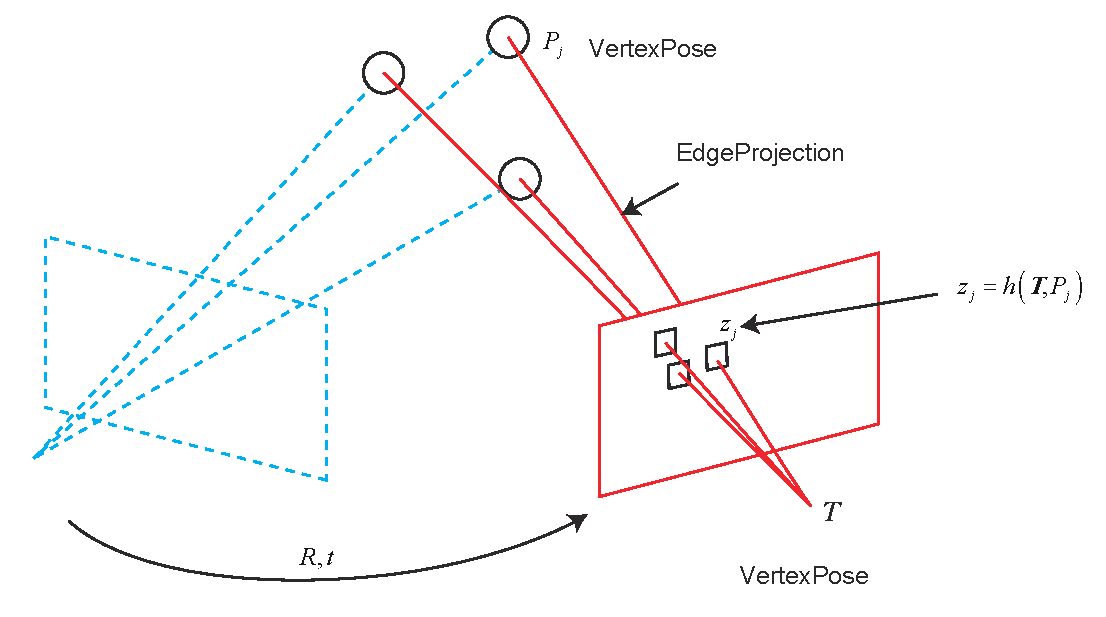
\includegraphics[width=0.9\linewidth]{vo1/ba-graph}
	\caption{PnP's graph structure.}
	\label{fig:ba-graph}
\end{figure}

In this graph optimization, the nodes and edges are defined as follows:
\begin{enumerate}
	\item \textbf{Node}: The pose of the second camera $\mathbf{T} \in \mathrm{SE}(3)$.
	\item \textbf{Edge}: The projection of each 3D point in the second camera, described by the observation equation:
	\[
	\mathbf{z}_j = h(\mathbf{T}, \mathbf{P}_{j}).
	\]
\end{enumerate}

Since the pose of the first camera is fixed to identity, we excluded it from the optimization variables. But in normal cases, we will consider estimations of many cameras. Now we estimate the second camera pose based on a set of 3D points and the 2D projection in the second image. We drew the first camera as a dotted line to indicate that we don't want to consider it.

g2o provides many nodes and edges about BA. For example, ``g2o/\\types/sba/types\_six\_dof\_expmap.h'' provides nodes and edges expressed by Lie algebra. In the second edition of the book, we implement a VertexPose vertex and EdgeProjection edge ourselves, as follows:
\begin{lstlisting}[language=c++,caption=slambook2/ch7/pose_estimation_3d2d.cpp (part)]
/// vertex and edges used in g2o ba
class VertexPose : public g2o::BaseVertex<6, Sophus::SE3d> {
	public:
	EIGEN_MAKE_ALIGNED_OPERATOR_NEW;
	
	virtual void setToOriginImpl() override {
		_estimate = Sophus::SE3d();
	}
	
	/// left multiplication on SE3
	virtual void oplusImpl(const double *update) override {
		Eigen::Matrix<double, 6, 1> update_eigen;
		update_eigen << update[0], update[1], update[2], update[3], update[4], update[5];
		_estimate = Sophus::SE3d::exp(update_eigen) * _estimate;
	}
	
	virtual bool read(istream &in) override {}
	
	virtual bool write(ostream &out) const override {}
};

class EdgeProjection : public g2o::BaseUnaryEdge<2, Eigen::Vector2d, VertexPose> {
	public:
	EIGEN_MAKE_ALIGNED_OPERATOR_NEW;
	
	EdgeProjection(const Eigen::Vector3d &pos, const Eigen::Matrix3d &K) : _pos3d(pos), _K(K) {}
	
	virtual void computeError() override {
		const VertexPose *v = static_cast<VertexPose *> (_vertices[0]);
		Sophus::SE3d T = v->estimate();
		Eigen::Vector3d pos_pixel = _K * (T * _pos3d);
		pos_pixel /= pos_pixel[2];
		_error = _measurement - pos_pixel.head<2>();
	}
	
	virtual void linearizeOplus() override {
		const VertexPose *v = static_cast<VertexPose *> (_vertices[0]);
		Sophus::SE3d T = v->estimate();
		Eigen::Vector3d pos_cam = T * _pos3d;
		double fx = _K(0, 0);
		double fy = _K(1, 1);
		double cx = _K(0, 2);
		double cy = _K(1, 2);
		double X = pos_cam[0];
		double Y = pos_cam[1];
		double Z = pos_cam[2];
		double Z2 = Z * Z;
		_jacobianOplusXi
		<< -fx / Z, 0, fx * X / Z2, fx * X * Y / Z2, -fx - fx * X * X / Z2, fx * Y / Z,
		0, -fy / Z, fy * Y / (Z * Z), fy + fy * Y * Y / Z2, -fy * X * Y / Z2, -fy * X / Z;
	}
	
	virtual bool read(istream &in) override {}
	
	virtual bool write(ostream &out) const override {}
	
	private:
	Eigen::Vector3d _pos3d;
	Eigen::Matrix3d _K;
};
\end{lstlisting}

This implements vertex update and edge error calculation. The following is to combine them into a graph optimization problem:
\begin{lstlisting}[language=c++,caption=slambook2/ch7/pose_estimation_3d2d.cpp (part)]
void bundleAdjustmentG2O(
const VecVector3d &points_3d,
const VecVector2d &points_2d,
const Mat &K,
Sophus::SE3d &pose) {
	// Build graph optimization, first let's define g2o
	typedef g2o::BlockSolver<g2o::BlockSolverTraits<6, 3>> BlockSolverType;  // pose is 6, landmark is 3
	typedef g2o::LinearSolverDense<BlockSolverType::PoseMatrixType> LinearSolverType;
	// Gradient descent method, you can choose from GN, LM, DogLeg
	auto solver = new g2o::OptimizationAlgorithmsGaussNewton(
		g2o::make_unique<BlockSolverType>(g2o::make_unique<LinearSolverType>()));
	g2o::SparseOptimizer optimizer;     // Graph model
	optimizer.setAlgorithm(solver);   // Set up the solver
	optimizer.setVerbose(true);       // Turn on verbose output for debugging
	
	// vertex
	VertexPose *vertex_pose = new VertexPose(); // camera vertex_pose
	vertex_pose->setId(0);
	vertex_pose->setEstimate(Sophus::SE3d());
	optimizer.addVertex(vertex_pose);
	
	// K
	Eigen::Matrix3d K_eigen;
	K_eigen <<
	K.at<double>(0, 0), K.at<double>(0, 1), K.at<double>(0, 2),
	K.at<double>(1, 0), K.at<double>(1, 1), K.at<double>(1, 2),
	K.at<double>(2, 0), K.at<double>(2, 1), K.at<double>(2, 2);
	
	// edges
	int index = 1;
	for (size_t i = 0; i < points_2d.size(); ++i) {
		auto p2d = points_2d[i];
		auto p3d = points_3d[i];
		EdgeProjection *edge = new EdgeProjection(p3d, K_eigen);
		edge->setId(index);
		edge->setVertex(0, vertex_pose);
		edge->setMeasurement(p2d);
		edge->setInformation(Eigen::Matrix2d::Identity());
		optimizer.addEdge(edge);
		index++;
	}
	
	chrono::steady_clock::time_point t1 = chrono::steady_clock::now();
	optimizer.setVerbose(true);
	optimizer.initializeOptimization();
	optimizer.optimize(10);
	chrono::steady_clock::time_point t2 = chrono::steady_clock::now();
	chrono::duration<double> time_used = chrono::duration_cast<chrono::duration<double>>(t2 - t1);
	cout << "optimization costs time: " << time_used.count() << " seconds." << endl;
	cout << "pose estimated by g2o =\n" << vertex_pose->estimate().matrix() << endl;
	pose = vertex_pose->estimate();
}
\end{lstlisting}

The program is similar to \textit{g2o} in lecture 6. We first declare the \textit{g2o} graph optimizer and configure the solver and gradient descent method. Then, based on the estimated feature points, we put the pose and spatial points into the graph. Finally, the optimization function is called. The partial output of the run is as follows:

\begin{lstlisting}[language=sh,caption=Terminal output:]
./build/pose_estimation_3d2d 1.png 2.png 1_depth.png 2_depth.png
-- Max dist : 95.000000 
-- Min dist : 4.000000 
In total, we get 79 set of feature points
3d-2d pairs: 76
solve pnp in opencv cost time: 0.000332991 seconds.
R=
[0.9978662025826269, -0.05167241613316376, 0.03991244360207524;
0.0505958915956335, 0.998339762771668, 0.02752769192381471;
-0.04126860182960625, -0.025449547736074, 0.998823919929363]
t=
[-0.1272259656955879;
-0.007507297652615337;
0.06138584177157709]
calling bundle adjustment by gauss newton
iteration 0 cost=645538.1857253
iteration 1 cost=12750.239874896
iteration 2 cost=12301.774589343
iteration 3 cost=12301.427574651
iteration 4 cost=12301.426806652
pose by g-n: 
0.99786618832  -0.0516873580423    0.039893448423   -0.127218696289
0.0506143671126    0.998340854865   0.0274540224544 -0.00738695798083
-0.0412462852904  -0.0253762590968    0.998826706403   0.0617019263823
0                 0                 0                 1
solve pnp by gauss newton cost time: 0.000159492 seconds.
calling bundle adjustment by g2o
iteration= 0	 chi2= 413.390599	 time= 2.7291e-05	 cumTime= 2.7291e-05	 edges= 76	 schur= 0	 lambda= 79.000412	 levenbergIter= 1
iteration= 1	 chi2= 301.367030	 time= 1.47e-05	 cumTime= 4.1991e-05	 edges= 76	 schur= 0	 lambda= 26.333471	 levenbergIter= 1
iteration= 2	 chi2= 301.365779	 time= 1.7794e-05	 cumTime= 5.9785e-05	 edges= 76	 schur= 0	 lambda= 17.555647	 levenbergIter= 1
iteration= 3	 chi2= 301.365779	 time= 1.4875e-05	 cumTime= 7.466e-05	 edges= 76	 schur= 0	 lambda= 11.703765	 levenbergIter= 1
iteration= 4	 chi2= 301.365779	 time= 1.3132e-05	 cumTime= 8.7792e-05	 edges= 76	 schur= 0	 lambda= 7.802510	 levenbergIter= 1
iteration= 5	 chi2= 301.365779	 time= 2.0379e-05	 cumTime= 0.000108171	 edges= 76	 schur= 0	 lambda= 41.613386	 levenbergIter= 3
iteration= 6	 chi2= 301.365779	 time= 3.4186e-05	 cumTime= 0.000142357	 edges= 76	 schur= 0	 lambda= 2859650082279.672363	 levenbergIter= 8
optimization costs time: 0.000763649 seconds.
pose estimated by g2o =
0.997866202583  -0.0516724161336   0.0399124436024   -0.127225965696
0.050595891596    0.998339762772   0.0275276919261 -0.00750729765631
-0.04126860183  -0.0254495477384    0.998823919929   0.0613858417711
0                 0                 0                 1
solve pnp by g2o cost time: 0.000923095 seconds.
\end{lstlisting}


Those three results are basically the same. In terms of efficiency, the Gauss-Newton method implemented by ourselves ranked first with 0.15 milliseconds, followed by OpenCV's PnP, and finally, the implementation of \textit{g2o}. Nonetheless, the time usages are all within 1 millisecond, which shows that the pose estimation algorithm does not really consume computational effort.

Bundle Adjustment is a common method rather than a special task. It may not be limited to two images. We can put the poses, and spatial points matched by multiple images for iterative optimization and even put the entire SLAM process in. We will deal with the large-scale problem again in lecture~\ref{cpt:9}. We usually consider a small bundle adjustment problem regarding local camera poses and feature points at the frontend, aiming to solve and optimize it in real-time.

\section{3D−3D:Iterative Closest Point (ICP)}
\label{sec:7.9}
In the end, we will introduce the 3D-3D pose estimation problem. Suppose we have a set of matched 3D points (for example, we matched two RGB-D images):
\[
\mathbf{P} = \{ \mathbf{p}_1, \cdots, \mathbf{p}_n \}, \quad \mathbf{P}' = \{ \mathbf{p}_1', \cdots, \mathbf{p}_n'\},
\]
Now, we want to find an Euclidean transformation $\mathbf{R}, \mathbf{t}$, which is \footnote{The notation in this section is slightly different from the symbols in the previous two sections. You can consider $\mathbf{p}_i$ as the data in the second image, and $\mathbf{p}_i'$ as the data in the first image, and consistently geting $ \mathbf{R},\mathbf{t}$.}:
\[
\forall i, \mathbf{p}_i = \mathbf{R} \mathbf{p}_i' + \mathbf{t}.
\]

This problem can be solved by the iterative closest point (ICP). The camera model does not appear in the 3D−3D pose estimation, meaning that when only the transformation between two sets of 3D points is considered, it has nothing to do with the camera. Therefore, ICP is also feasible in lidar SLAM. But since lidar features are not rich enough, it is hard to know the matching relationship between the two pointsets.  We can only assume the closest points are the same. So this method is called the iterative closest point. The feature points provide us with a better matching relationship in the computer vision, so the whole problem becomes easier to solve. In RGB-D SLAM, the camera pose can also be estimated in this way. In the following, we use ICP to refer to the motion estimation problem between the two sets of \textbf{matched} points.

Similar to PnP, the solution to ICP can be divided into two ways: using linear algebra (mainly SVD) and using nonlinear optimization (similar to Bundle Adjustment). They will be introduced separately below.

\subsection{Using Linear Algebra (SVD)}
First, let's look at the SVD on behalf of the algebraic method. According to the ICP problem described above, we first define the error term for the point $i$ as:
\begin{equation}
\mathbf{e}_i = \mathbf{p}_i - (\mathbf{R} \mathbf{p}_i' + \mathbf{t} ) .
\end{equation}

Then, construct a least-square problem to find the $\mathbf{R}, \mathbf{t}$ by minimization of sum of the squared errors:
\begin{equation}
\mathop {\min }\limits_{\mathbf{R}, \mathbf{t}} \frac{1}{2} \sum\limits_{i = 1}^n\| {\left( {{\mathbf{p}_i} - \left( {\mathbf{R}{\mathbf{p}_i}' + \mathbf{t}} \right)} \right)} \|^2_2.
\end{equation}

To solve this problem, we define the centroids of the two sets of points as:
\begin{equation}
\mathbf{p} = \frac{1}{n}\sum_{i=1}^n ( \mathbf{p}_i ), \quad \mathbf{p}' = \frac{1}{n} \sum_{i=1}^n ( \mathbf{p}_i' ). 
\end{equation}

The centroids are not subscripted. Then, in the error function:
\begin{align*}
\begin{array}{ll}
\frac{1}{2}\sum\limits_{i = 1}^n {{{\left\| {{\mathbf{p}_i} - \left( {\mathbf{R}{ \mathbf{p}_i}' + \mathbf{t}} \right)} \right\|}^2}}  & = \frac{1}{2}\sum\limits_{i = 1}^n {{{\left\| {{\mathbf{p}_i} - \mathbf{R}{\mathbf{p}_i}' - \mathbf{t} - \mathbf{p} + \mathbf{Rp}' + \mathbf{p} - \mathbf{Rp}'} \right\|}^2}} \\
 & = \frac{1}{2}\sum\limits_{i = 1}^n {{{\left\| {\left( {{\mathbf{p}_i} - \mathbf{p} - \mathbf{R}\left( {{\mathbf{p}_i}' - \mathbf{p}'} \right)} \right) + \left( {\mathbf{p} - \mathbf{Rp}' - \mathbf{t}} \right)} \right\|}^2}} \\
& = \frac{1}{2}\sum\limits_{i = 1}^n ( {{\left\| {{\mathbf{p}_i} - \mathbf{p} - \mathbf{R}\left( {{\mathbf{p}_i}' - \mathbf{p}'} \right)} \right\|}^2} + {{\left\| {\mathbf{p} - \mathbf{Rp}' - \mathbf{t}} \right\|}^2} +\\
 & \quad \quad 2{{\left( {{\mathbf{p}_i} - \mathbf{p} - \mathbf{R}\left( {{\mathbf{p}_i}' - \mathbf{p}'} \right)} \right)}^T}\left( {\mathbf{p} - \mathbf{Rp}' - \mathbf{t}} \right)). 
\end{array}
\end{align*}

Since $\left( {{\mathbf{p}_i} - \mathbf{p} - \mathbf{R}\left( {{\mathbf{p}_i}' - \mathbf{p}'} \right)} \right)$ is zero after the summation, so the optimization objective function can be simplified to
\begin{equation}
\mathop {\min }\limits_{\mathbf{R}, \mathbf{t}} J = \frac{1}{2}\sum\limits_{i = 1}^n {{\left\| {{\mathbf{p}_i} - \mathbf{p} - \mathbf{R}\left( {{\mathbf{p}_i}' - \mathbf{p}'} \right)} \right\|}^2} + {{\left\| {\mathbf{p} - \mathbf{Rp}' - \mathbf{t}} \right\|}^2} .
\end{equation}

Carefully observe those two terms, we find that the first term is only related to the rotation matrix $\mathbf{R}$, while the second has both $\mathbf{R}$ and $\mathbf{t}$, but only related to the centroid. As long as we get $\mathbf{R}$, we can get $\mathbf{t}$ by making the second term zero. Therefore, ICP can be solved in the following three steps:

\begin{mdframed}
\begin{enumerate}
	\item Calculate the centroids of the two groups of points $\mathbf{p}, \mathbf{p}'$, and then calculate the \textbf{de-centroid coordinates} of each point:
	\[
	\mathbf{q}_i = \mathbf{p}_i - \mathbf{p}, \quad \mathbf{q}_i' = \mathbf{p}_i' - \mathbf{p}'.
	\]
	\item The rotation matrix is calculated according to the following optimization problem:
	\begin{equation}
		\mathbf{R}^* = \arg \mathop {\min }\limits_{\mathbf{R}} \frac{1}{2}\sum\limits_{i = 1}^n {{\left\| {{\mathbf{q}_i} - \mathbf{R} \mathbf{q}_i' } \right\|}^2}.
	\end{equation}
	\item Calculate $\mathbf{t}$ according to $\mathbf{R}$ in step 2:
	\begin{equation}
	\label{eq:pnp-solve-t}
	\mathbf{t}^* = \mathbf{p} - \mathbf{R} \mathbf{p}'.
	\end{equation}
\end{enumerate}
\end{mdframed}

We find that once the rotation between the two sets of points is found, and the translation is easy to obtain. So we focus on the calculation of $\mathbf{R}$. Expand the error term about $\mathbf{R}$, we get:
\begin{equation}
 \frac{1}{2}\sum\limits_{i = 1}^n \left\| {{\mathbf{q}_i} - \mathbf{R} \mathbf{q}_i' } \right\|^2 = \frac{1}{2}\sum\limits_{i = 1}^n \underbrace{\mathbf{q}_i^T \mathbf{q}_i}_{\text{not relavant}} + \mathbf{q}_i^{ \prime \mathrm{T}} \underbrace{\mathbf{R}^T \mathbf{R}}_{=\mathbf{I}} \mathbf{q}^\prime_i - 2\mathbf{q}_i^T \mathbf{R} \mathbf{q}^\prime_i.
\end{equation}

The first item is not relevant to $\mathbf{R}$. The second item can also be ignored since $\mathbf{R}^T\mathbf{R}=\mathbf{I}$. Therefore, the actual optimization objective function becomes the form of:
\begin{equation}
\sum\limits_{i = 1}^n - \mathbf{q}_i^T \mathbf{R} \mathbf{q}^\prime_i = \sum\limits_{i = 1}^n -\mathrm{tr} \left( \mathbf{R} \mathbf{q}_i^{\prime} \mathbf{q}^T_i \right) = - \mathrm{tr} \left( \mathbf{R} \sum\limits_{i = 1}^n \mathbf{q}_i^{\prime} \mathbf{q}^T_i \ \right).
\end{equation}

Next, we introduce how to solve the optimal $\mathbf{R}$ in the above problem through SVD. The proof of optimality is more complicated, and interested readers can refer to the literature~\cite{Arun1987, PomerleauColasSiegwart2015}. To find $\mathbf{R}$, first define the matrix:
\begin{equation}
\mathbf{W} =  \sum\limits_{i = 1}^n \mathbf{q}_i \mathbf{q}^{\prime \mathrm{T}}_i.
\end{equation}

$\mathbf{W}$ is a $3 \times 3$ matrix. Performing SVD decomposition on $\mathbf{W}$, we get:
\begin{equation}
\mathbf{W} = \mathbf{U} \boldsymbol{\Sigma} \mathbf{V}^T.
\end{equation}

$\boldsymbol{\Sigma}$ is a diagonal matrix composed of singular values, the diagonal elements are arranged from large to small, and $\mathbf{U}$, $\mathbf{V}$ are diagonal matrices. When $\mathbf{W}$ is of full rank, $\mathbf{R}$ is:
\begin{equation}
\mathbf{R} = \mathbf{U} \mathbf{V}^T.
\end{equation}

Once solving $\mathbf{R}$, we can use the equation \eqref{eq:pnp-solve-t} to solve $\mathbf{t}$. If the determinant of $\mathbf{R}$ is negative, then $-\mathbf{R}$ is taken as the optimal value.

\subsection{Using non-linear optimization}
Another way to solve ICP is to use nonlinear optimization to find the optimal value iteratively. This method is similar to the PnP we described earlier. When expressing the poses in Lie algebra, the objective function can be written as
\begin{equation}
\mathop {\min }\limits_{\boldsymbol{\xi}} = \frac{1}{2} \sum\limits_{i = 1}^n\| {\left( {{{\mathbf{p}}_i} - \exp \left( \boldsymbol{\xi}^\wedge \right) {\mathbf{p}}'_i} \right)} \|^2_2.
\end{equation}

The derivative of a single error term with respect to the pose has been derived above, using the Lie algebra perturbation model:
\begin{equation}
\frac{{\partial \mathbf{e}}}{{\partial \delta \boldsymbol{\xi} }} =  - {\left( {\exp \left( {{ \boldsymbol{\xi} ^ \wedge }} \right){{\mathbf{p}}_i}'} \right)^ \odot }.
\end{equation}

Therefore, in nonlinear optimization, it only needs to iterate continuously to find the minimum value. Moreover, it can be proved that  {\cite{Barfoot2016}} the ICP problem has a unique solution or an infinite number of solutions. In the case of a unique solution, as long as the minimum value solution can be found, this minimum value is the global minimum. This also means that the initial value of the ICP solution can be arbitrarily selected. This is a big advantage of solving ICP when the points have been matched already.

It should be noted that the ICP we are talking about here refers to the problem of pose estimation when the matching is given by the image features. In the case of known matching, this least-squares problem actually has an analytical solution  {\cite{Faugeras1986, Horn1987, Sharp2002}}, so iterative optimization is not necessary. ICP researchers tend to be more concerned about the unknown matching situation. So, why do we introduce optimization-based ICP? Because in some cases, such as in RGB-D SLAM, the depth of a pixel may or may not be measured, so we can combine PnP and ICP optimization. For feature points with known depth, model their 3D-3D errors; for feature points with unknown depths, model 3D-2D reprojection errors. Therefore, all errors can be considered in the same problem, making the solution more convenient.

\section{Practice: Solving ICP}
\subsection{Using SVD}
Let's demonstrate how to use SVD and nonlinear optimization to solve ICP. In this section, we use two RGB-D images to obtain two sets of 3D points through feature matching, and finally, we use ICP to calculate their pose transformation. Since OpenCV does not currently have a method to calculate two sets of ICPs with matching points, and its principle is not complicated, we will implement an ICP by ourselves.
\begin{lstlisting}[language=c++,caption=slambook2/ch7/pose\_estimation\_3d3d.cpp (part)]
void pose_estimation_3d3d(
const vector<Point3f> &pts1,
const vector<Point3f> &pts2,
Mat &R, Mat &t) {
	Point3f p1, p2;     // center of mass
	int N = pts1.size();
	for (int i = 0; i < N; i++) {
		p1 += pts1[i];
		p2 += pts2[i];
	}
	p1 = Point3f(Vec3f(p1) / N);
	p2 = Point3f(Vec3f(p2) / N);
	vector<Point3f> q1(N), q2(N); // remove the center
	for (int i = 0; i < N; i++) {
		q1[i] = pts1[i] - p1;
		q2[i] = pts2[i] - p2;
	}
	
	// compute q1*q2^T
	Eigen::Matrix3d W = Eigen::Matrix3d::Zero();
	for (int i = 0; i < N; i++) {
		W += Eigen::Vector3d(q1[i].x, q1[i].y, q1[i].z) * Eigen::Vector3d(q2[i].x, q2[i].y, q2[i].z).transpose();
	}
	cout << "W=" << W << endl;
	
	// SVD on W
	Eigen::JacobiSVD<Eigen::Matrix3d> svd(W, Eigen::ComputeFullU | Eigen::ComputeFullV);
	Eigen::Matrix3d U = svd.matrixU();
	Eigen::Matrix3d V = svd.matrixV();
	
	cout << "U=" << U << endl;
	cout << "V=" << V << endl;
	
	Eigen::Matrix3d R_ = U * (V.transpose());
	if (R_.determinant() < 0) {
		R_ = -R_;
	}
	Eigen::Vector3d t_ = Eigen::Vector3d(p1.x, p1.y, p1.z) - R_ * Eigen::Vector3d(p2.x, p2.y, p2.z);
	
	// convert to cv::Mat
	R = (Mat_<double>(3, 3) <<
		R_(0, 0), R_(0, 1), R_(0, 2),
		R_(1, 0), R_(1, 1), R_(1, 2),
		R_(2, 0), R_(2, 1), R_(2, 2)
	);
	t = (Mat_<double>(3, 1) << t_(0, 0), t_(1, 0), t_(2, 0));
}
\end{lstlisting}

The implementation of ICP is consistent with the previous theoretical part. We call \textit{Eigen} for SVD and then calculate the $\mathbf{R}, \mathbf{t}$ matrix. We output the matched result, but please note that since the previous derivation is based on $\mathbf{p}_i = \mathbf{R} \mathbf{p}_i' + \mathbf{t}$, here is $\mathbf{R}, \mathbf{t}$ is the transformation from the second frame to the first frame, which is the opposite of the previous theoritical part. So in the output result, we also printed the inverse transform:

\begin{lstlisting}[language=sh,caption=Terminal output:]
./build/pose_estimation_3d3d 1.png 2.png 1_depth.png 2_depth.png
-- Max dist : 95.000000 
-- Min dist : 4.000000 
In total, we get 79 set of feature points
3d-3d pairs: 74
W=  11.9404 -0.567258   1.64182
-1.79283   4.31299  -6.57615
3.12791  -6.55815   10.8576
U=  0.474144  -0.880373 -0.0114952
-0.460275  -0.258979   0.849163
0.750556   0.397334   0.528006
V=  0.535211  -0.844064 -0.0332488
-0.434767  -0.309001    0.84587
0.724242   0.438263   0.532352
ICP via SVD results: 
R = [0.9972395977366739, 0.05617039856770099, -0.04855997354553433;
-0.05598345194682017, 0.9984181427731508, 0.005202431117423125;
0.0487753812298326, -0.002469515369266572, 0.9988067198811421]
t = [0.1417248739257469;
-0.05551033302525193;
-0.03119093188273858]
R_inv = [0.9972395977366739, -0.05598345194682017, 0.0487753812298326;
0.05617039856770099, 0.9984181427731508, -0.002469515369266572;
-0.04855997354553433, 0.005202431117423125, 0.9988067198811421]
t_inv = [-0.1429199667309695;
0.04738475446275858;
0.03832465717628181]
\end{lstlisting}

Readers can compare the difference between ICP and PnP and the motion estimation results of epipolar geometry. We are using more and more information in this process (no depth $\rightarrow$ the depth of one image $\rightarrow$ the depth of two images). Therefore, when the depth is accurate, the estimates will be more and more accurate. However, due to the noise in Kinect's depth map and the possibility of data loss, we have to discard some feature points without depth data. This may cause the estimation of ICP to be inaccurate, and if too many feature points are discarded, it may cause a situation where motion estimation cannot be performed due to too few feature points.

\subsection{Using non-linear optimization}
Now consider using nonlinear optimization to calculate ICP. We still use Lie algebra to optimize the camera pose. The RGB-D camera can observe the 3D position of the landmarks every time, thereby generating 3D observation data. We use the VertexPose in the previous practice and then define the unary edges of 3D-3D:
\begin{lstlisting}[language=c++,caption=slambook2/ch7/pose\_estimation\_3d3d.cpp (part)]
/// g2o edge
class EdgeProjectXYZRGBDPoseOnly : public g2o::BaseUnaryEdge<3, Eigen::Vector3d, VertexPose> {
public:
	EIGEN_MAKE_ALIGNED_OPERATOR_NEW;
	
	EdgeProjectXYZRGBDPoseOnly(const Eigen::Vector3d &point) : _point(point) {}
	
	virtual void computeError() override {
		const VertexPose *pose = static_cast<const VertexPose *> ( _vertices[0] );
		_error = _measurement - pose->estimate() * _point;
	}
	
	virtual void linearizeOplus() override {
		VertexPose *pose = static_cast<VertexPose *>(_vertices[0]);
		Sophus::SE3d T = pose->estimate();
		Eigen::Vector3d xyz_trans = T * _point;
		_jacobianOplusXi.block<3, 3>(0, 0) = -Eigen::Matrix3d::Identity();
		_jacobianOplusXi.block<3, 3>(0, 3) = Sophus::SO3d::hat(xyz_trans);
	}
	
	bool read(istream &in) {}
	
	bool write(ostream &out) const {}
	
protected:
	Eigen::Vector3d _point;
};
\end{lstlisting}

They are unary edges, similar to the g2o::EdgeSE3ProjectXYZ mentioned earlier, but the observation has changed from 2 to 3 dimensions. There is no camera model involved, and only one vertex is related. Please pay attention to the form of the Jacobian matrix here. It must be consistent with our previous derivation. The Jacobian matrix gives the derivative of the camera pose and is $3 \times 6$.

The code for using \textit{g2o} for optimization is similar. We just set the nodes and edges for graph optimization. Readers are suggested to check the source file for this part of the code, which is not listed here. Now, let’s take a look at the results of the optimization:

\begin{lstlisting}[language=sh, caption=Terminal output:]
iteration= 0	 chi2= 1.811539	 time= 1.7046e-05	 cumTime= 1.7046e-05	 edges= 74	 schur= 0
iteration= 1	 chi2= 1.811051	 time= 1.0422e-05	 cumTime= 2.7468e-05	 edges= 74	 schur= 0
iteration= 2	 chi2= 1.811050	 time= 9.589e-06	 cumTime= 3.7057e-05	 edges= 74	 schur= 0
...中间略
iteration= 9	 chi2= 1.811050	 time= 9.113e-06	 cumTime= 0.000100604	 edges= 74	 schur= 0
optimization costs time: 0.000559208 seconds.

after optimization:
T=
0.99724  0.0561704   -0.04856   0.141725
-0.0559834   0.998418 0.00520242 -0.0555103
0.0487754 -0.0024695   0.998807 -0.0311913
0          0          0          1
\end{lstlisting}

We found that the overall error has become stable after only one iteration, indicating that the algorithm has converged after only one iteration. From the result of the pose, it can be seen that it is almost the same as the pose calculated by the previous SVD, which shows that SVD has already given an analytical solution to the optimization problem. Therefore, in this practice, it can be considered that the result given by SVD is the optimal value of the camera pose.

It should be noted that in the practice of ICP, we used feature points that have depth readings in both images. However, as long as the depth of one of the images is determined, we can use errors similar to PnP to add them to the optimization. In addition to the camera pose, considering the spatial points as optimization variables is also a way to solve it. We should be clear that the actual solution is very flexible and does not need to be bound to a certain fixed form. If you consider points and cameras simultaneously, the whole problem becomes more flexible, and you may get other solutions. For example, you can make the camera rotate less and move the point more. This reflects that we would like to have as many constraints as possible in bundle adjustment because multiple observations will bring more information and enable us to estimate each variable more accurately.

\section{Summary}
This chapter introduces several important issues in visual odometry based on feature points, including:

\begin{enumerate}
	\item How the feature points are extracted and matched.
	\item How to estimate camera motion through 2D-2D feature points.
	\item How to estimate the spatial position of a point from a 2D−2D match.
	\item 3D−2D PnP problem and its linear solution and bundle adjustment solution.
	\item 3D−3D ICP problem and its linear solution and bundle adjustment solution.
\end{enumerate}

This chapter is complicated in content and combines the basic knowledge of the previous lectures. If readers find it difficult to understand, please go back to review the previous chapters. It is best to do the practice yourself to entirely understand the content of the motion estimation.

What needs to be mentioned here is we have omitted a lot of discussion about some special situations. For example, what happens if the given feature points are coplanar during the epipolar geometry solution (this is mentioned in the homography matrix $\mathbf{H}$)? What happens to collinear? If we solve such a solution in PnP and ICP, what will happen? Can the algorithms recognize these exceptional cases and report that the resulting solution may be unreliable? Can you give the estimated uncertainty of $\mathbf{T}$? Although they are all worthy of research and exploration, their discussion is more suitable in specific papers. The goal of this book is to cover basic knowledge of visual SLAM. We will not expand on these issues for now. At the same time, these situations rarely occur in engineering. If you care about these rare situations, you can read books such as~\cite{Hartley2003}.

\section*{Exercises}
\begin{enumerate}
	\item In addition to the ORB feature points introduced in this book, what other feature points do you know? Please elaborate on the principles of SIFT or SURF, and compare their advantages and disadvantages with ORB.
	\item Write a program to call other types of feature points in OpenCV. Compare their time spent on your machine when extracting 1000 feature points.
	\item[\optional] We found that the ORB feature points provided by OpenCV are not evenly distributed in the image. Can you find or propose a way to make the distribution of feature points more evenly?
	\item Investigate why FLANN can quickly handle matching problems. In addition to FLANN, what other ways to accelerate matching?
	\item Substitute the EPnP used in the demo program with other PnP methods and investigate their working principles.
	\item In PnP optimization, taking the first camera's observation into consideration, how should the problem/program be formed? How will the final result change?
	\item In the ICP program, if the spatial points are also considered optimization variables, how should the program be written? How will the final result change?
	\item[\optional] In the feature point matching, mismatches will inevitably be encountered. What happens if we put the wrong match into PnP or ICP? What methods can you think of to avoid mismatches?
	\item[\optional] Use the SE3 class in Sophus to write the nodes and edges of \textit{g2o} by yourself and implement the optimization of PnP and ICP.
	\item[\optional] Implement the optimization of PnP and ICP in Ceres.
\end{enumerate}

%\section*{Depth Filter}
%Using the above linear solution triangulation method, the 3D point coordinates obtained are always uncertain, and multiple measurements of the same point will often estimate different depths. Affected by noise, when the baseline is shorter, the depth is more sensitive to noise. Therefore, we need to reduce the error contained in a single measurement solution. The depth filter measures the same map point multiple times to continuously approach the true depth of the map point, which is a very effective method.~\cite{vogiatzis2011video}\par
%The core concept is that a valid depth measurement value $d_{n}$ has a Gaussian distribution around the real depth $D$, while an invalid measurement value $d_{bad}$ is uniformly distributed in a certain depth range$[ D_{min},D_{max}]$, and the probability that the measured value is valid is $\alpha$. The probability distribution function is:
%\begin{equation}
%p(d_{n}|D,\alpha)=\alpha N(d_{n}|D,\tau_{n}^{2})+(1-\alpha)U(d_{bad}|D_{min},D_{max})
%\end{equation}
%Our goal is to approximate the true depth $D$ through multiple measurements $d_{n}$. Every time we have a new measurement $d_{n+1}$, the parameters of the probability model are adjusted accordingly. \par
%
%If there are N sets of measurements, assuming that each measurement is independent of each other, it can be obtained by the Bayesian formula:
%\begin{equation}
%p(D,\alpha|x_{1},x_{2},...,x_{N}) \propto p(D,\alpha) \prod_{n}p(d_{n}|D,\alpha)
%\end{equation}
%
%$p(D,\alpha)$ is a prior distribution, assuming that the two are independent of each other, that is, $p(D,\alpha)=p(D)p(\alpha)$.
%
% Now introduce a binary latent variable $y_{n}$ into the model, $y_{n}=1$ indicates that the measured value is valid, and vice versa. So there are:
%$$
%p(d_{n}|D,\alpha,y_{n}=N(d_{n}|D,\tau_{n}^{2})^{y_{n}}U(x_{n})^{1-y_{n}}
%$$
%$$
%p(y_{n}|\alpha)=\alpha^{y_{n}}(1-\alpha)^{1-y_{n}}
%$$
%
%
%\begin{equation}
%p(d,y,D,\alpha)=\prod_{n=1}^{N}p(d_{n}|D,\alpha,y_{n})p(y_{n}|\alpha) p(D)p(\alpha)
%\end{equation}
%
%Now, we need to approximately express the posterior probability $p(y,D,\alpha|d)$. Find an approximate distribution $q(y,D,\alpha)$, which has the smallest KL divergence with the real $p(y,D,\alpha|d)$.
%
%\begin{equation}
%q(D,\alpha)=\prod_{n=1}^{N}N(d_{n}|D,\sigma^{2})^{r_{n}}\alpha^{S}(1-\alpha)^{N-S}p(D)p(\alpha)
%\end{equation}
%
%$r_{n}=E_{y}[y_{n}]$ is the valid expectation of the $n$th measured value, and $S=\sum_{n=1}^{N}r_{n}$ . \par
%
% This probability distribution function is the product of a normal distribution and a Bernoulli distribution. Since the conjugate prior function of the normal distribution is still a normal distribution, the conjugate prior of the Bernoulli distribution is a Beta function, so The above formula can be transformed into:
%\begin{equation}
%q(D,\alpha|a,b,\mu,\sigma^{2})=N(D|\mu,\sigma^{2})Beta(\alpha|a,b)
%\end{equation}
%
%So the posterior update equation is:
%\begin{equation}
%q(D,\alpha|a',b',\mu',\sigma'^{2})=p(x|D,\alpha)q(D,\alpha|a,b,\mu,\sigma^{2})
%\end{equation}
%
%
%Substitute it into the previous equation:
%\begin{eqnarray}
%\begin{split}
%&(\alpha N(d|D,\tau^{2})+(1-\alpha)U(d))N(D|\mu,\sigma^{2})Beta(\alpha|a,b)\\
%=&\frac{a}{a+b}N(d|\mu,\sigma^{2}+\tau^{2})N(D|m,s^{2})Beta(\alpha|a+1,b)+\\
%&\frac{b}{a+b}U(d)N(D|\mu,\sigma^{2})Beta(\alpha|a,b+1)
%\end{split}
%\end{eqnarray}
%
%In the above equation, $\frac{1}{s^{2}}=\frac{\mu}{\sigma^{2}}+\frac{d}{\tau^{2}}$,$m=s^{2}(\frac{\mu}{\sigma^{2}}+\frac{d}{\tau^{2}})$,$C_{1}=\frac{a}{a+b}N(d|\mu,\sigma^{2}+\tau^{2})$, $C_{2}=\frac{b}{a+b}U(d)$。
%
%Using the method of moment estimation, estimate the first and second moments of $D$ and $\alpha$ respectively:
%
%\begin{eqnarray}
%\begin{split}
%&u'=C_{1}m+C_{2}\mu\\
%&\sigma'^{2}+\mu'^{2}=C_{1}(s^{2}+m^{2})+C_{2}(\sigma^{2}+\mu^{2})\\
%&\frac{a'}{a'+b'}=C_{1}\frac{a+1}{a+b+1}+C_{2}\frac{a}{a+b+1}\\
%&\frac{a'(a'+1)}{(a'+b')(a'+b'+1)}=C_{1}\frac{(a+1)(a+2)}{(a+b+1)(a+b+2)}+C_{2}\frac{a(a+1)}{(a+b+1)(a+b+2)}
%\end{split}
%\end{eqnarray}
% Combine the above equations to solve the updated model parameters $a',b',\sigma',\mu'$.
%
%\begin{figure}[!htp]
%    \centering
%    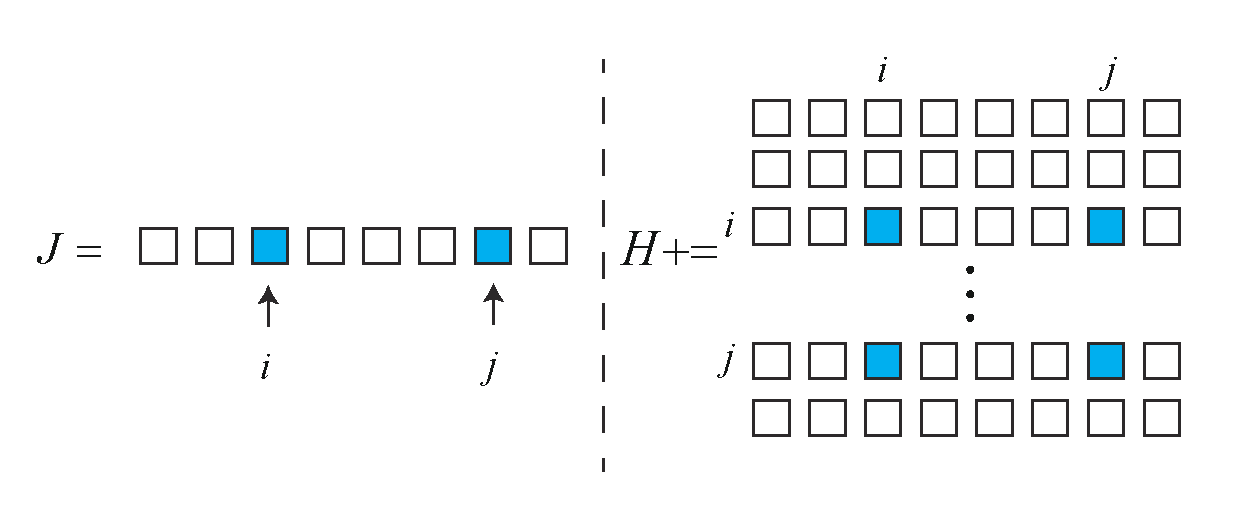
\includegraphics[width=0.3\linewidth]{vo1/sparse}
%    \includegraphics[width=0.3\linewidth]{vo1/semidense}
%    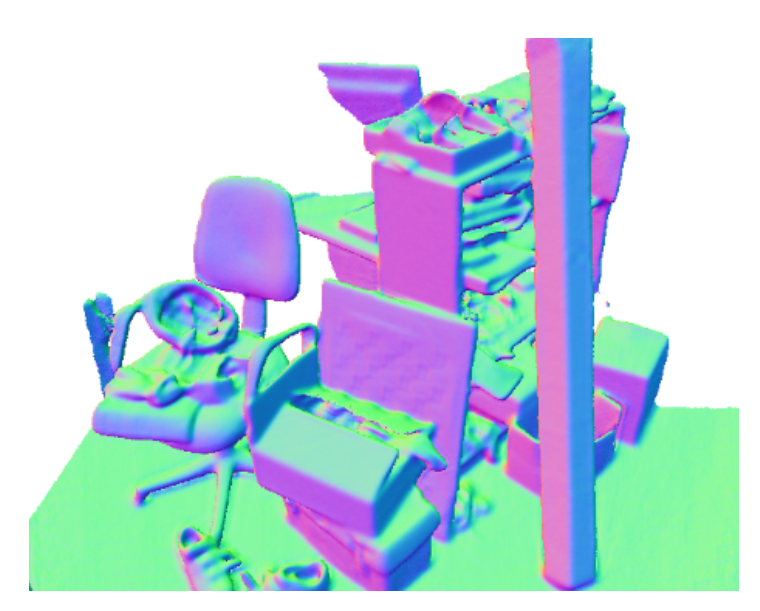
\includegraphics[width=0.3\linewidth]{vo1/dense}
%    \caption{Sparse map, semi-dense map and dense map}
%    \label{fig:threemethods}
%\end{figure}